\documentclass[twocolumn,10pt]{article}
\usepackage[margin=0.66in,top=0.70in,bottom=0.74in,columnsep=0.23in]{geometry}
\usepackage{amsmath,amssymb}
\usepackage{booktabs}
\usepackage{array}
\usepackage{graphicx}
\usepackage{xcolor}
\usepackage{caption}
\usepackage{fancyhdr}
\usepackage{hyperref}

\setlength{\emergencystretch}{1.6em}
\renewcommand{\topfraction}{0.92}
\renewcommand{\bottomfraction}{0.85}
\renewcommand{\textfraction}{0.08}
\renewcommand{\floatpagefraction}{0.85}
\raggedbottom

\definecolor{linkblue}{HTML}{124E78}

\captionsetup{font=small,labelfont=bf,skip=4pt}

\hypersetup{
  colorlinks=true,
  linkcolor=linkblue,
  citecolor=linkblue,
  urlcolor=linkblue,
  pdftitle={An All-Sky Prospectively Locked Panchromatic (0.38-2.515 um) Echelle Laser and Frequency-Comb Survey Across 150 Stellar Systems and a 160-System Multi-Messenger SETI Synthesis},
  pdfauthor={Martin Andersen}
}

\pagestyle{fancy}
\fancyhf{}
\fancyhead[L]{\footnotesize\textcolor{gray}{Andersen (2026) --- 150-Star All-Sky Echelle Laser \& Comb Survey (0.38--2.515\,$\mu$m) \& 160-System Multi-Messenger SETI Synthesis}}
\fancyhead[R]{\footnotesize\textcolor{gray}{\thepage}}
\renewcommand{\headrulewidth}{0.3pt}
\setlength{\headheight}{13pt}

\title{\vspace{-0.9em}\textbf{\Large An All-Sky Prospectively Locked Panchromatic (0.38--2.515\,$\mu$m) Echelle Laser and Frequency-Comb Survey Across 150 Stellar Systems with Seven Spectrographs and a 160-System Multi-Messenger SETI Synthesis}}
\author{\textbf{Martin Andersen}\\[0.2em]
\small MSc Astrophysics, University of Copenhagen\\
\small Public Code, Locked Protocols \& Audit Ledgers: \href{https://github.com/andersenmartin-blip/setisearch}{https://github.com/andersenmartin-blip/setisearch}}
\date{\small 17 November 2026}

\begin{document}

\twocolumn[
\begin{@twocolumnfalse}
\maketitle
\vspace{-0.9em}
\begin{abstract}
\noindent High-resolution astronomical echelle spectrographs built for extreme-precision radial-velocity exoplanet discovery simultaneously act as sensitive receivers for narrowband continuous-wave (CW) interstellar lasers and periodic optical/infrared frequency combs, yet archival searches have historically suffered from thousands of photospheric, telluric/OH airglow, detector, and orbital Doppler-smearing false positives. Here we present a unified, prospectively locked seven-phase panchromatic ($0.38\text{--}2.515\,\mu\text{m}$) all-sky laser and frequency-comb technosignature survey (\textbf{Phases D079--D085}, \texttt{V3.0-V4.0}) across \textbf{seven spectrographs} (ESO \textbf{HARPS}, VLT \textbf{ESPRESSO}, La Silla \textbf{NIRPS\_HE}, VLT \textbf{CRIRES+}, TNG \textbf{HARPS-N}, Calar Alto \textbf{CARMENES\_VIS}, and CFHT 3.6\,m \textbf{SPIRou} APERO \texttt{0.7.295}), \textbf{150 unique stellar systems} ($106$ South + $44$ North), and \textbf{1,009 archival exposures} ($195.23\,\text{h}$ integration; $221.66\times 10^{6}$ searched 1D bins plus $20.92\times 10^{6}$ \texttt{COMB\_V4} comb configurations). Every cohort list and gate threshold was SHA-256 sealed prior to science FITS ingestion and independently verified via pure Python standard-library audits.\par\smallskip
\noindent Across \textbf{13,284 synthetic control trials} ($8{,}541$ in \texttt{D079-D083}, $2{,}151$ in \texttt{D084}, and $2{,}592$ in \texttt{D085}), our five-channel pipeline (\textbf{T}, \textbf{P}, \textbf{T\_DIFF}, Keplerian \textbf{K\_PLANET}, and \texttt{COMB\_V4} periodic comb matched filtering) achieves $93.3\%\text{--}94.4\%$ southern optical, $91.3\%$ northern clean optical ($532\text{--}670\,\text{nm}$), $90.9\%$ NIRPS YJH, $78.9\%$ CRIRES+ $K$-band ($94.4\%$ Ho:YAG), and $85.5\%$ SPIRou YJHK ($95.8\%$ at $1064.1$ and $1662.0\,\text{nm}$) single-epoch $8\sigma$ completeness. In \texttt{D085} (\texttt{SPIROU\_V3\_6\_AND\_COMB\_V4}), upgrading cross-star Gate \texttt{G6\_V35} to the sparse $4{,}472$-peak supraphotospheric atlas \texttt{G6\_V36} ($11.154\times$ compression vs.\ $49{,}880$ peaks) lifts true-laser pass completeness from $50.0\%$ to \textbf{95.0\%} while keeping \textbf{100.0\%} sky-OH, H4RG warm-pixel, and intra-star BERV-stationary rejection, and \texttt{COMB\_V4} achieves \textbf{97.2\%} 6-tooth comb recovery ($\ge 3.8\sigma$/tooth) with $0.0\%$ single-line ($0/48$) and $2.2\%$ ($1/45$) pseudo-comb false-positive rates. Across all 1,009 exposures and 40 multi-epoch campaigns, \texttt{V3-V4} collapses \textbf{12,107 Legacy V2 false alarms} ($4{,}044$ in \texttt{D085}) to \textbf{0 orbital hits} and---after forensic closure of all 113 post-\texttt{G6\_V36} single-line and 19 \texttt{COMB\_V4} candidates in \texttt{D085}---\textbf{0 verified ETI detections} across all 150 stars (124 science hosts including 93 planet hosts with 183 planets, plus 26 zero-planet controls). Adding SPIRou closes the CARMENES VIS $>995\,\text{nm}$ dichroic sensitivity drop by $16\text{--}51\times$ (\textbf{730.5\,W} on DX\,Cnc at $1310\,\text{nm}$, \textbf{736\,W} at $1064.1\,\text{nm}$; \textbf{972.7\,W} on Wolf\,359; \textbf{718\,W} orbital on GJ\,1002\,b), establishing a \textbf{2.37\,kW} median across \textbf{73} $<10\,\text{pc}$ \textbf{stars} ($57$ science + $16$ controls; down to \textbf{9.03\,W} on Proxima Cen) and a \textbf{160-system multi-messenger synthesis} (\textbf{14 direct overlap hosts} adding $\rho$\,CrB / \texttt{M20}) with \textbf{0 verified ETI detections}.\par\smallskip
\noindent\textbf{Keywords:} extraterrestrial intelligence (SETI) --- technosignatures --- instrumentation: spectrographs --- infrared: stars --- radio continuum: planetary systems --- solar neighborhood --- optical frequency combs
\end{abstract}
\vspace{0.8em}
\hrule
\vspace{1.0em}
\end{@twocolumnfalse}
]
\thispagestyle{plain}

\section{Introduction}
Since Schwartz \& Townes \cite{SchwartzTownes1961} demonstrated that diffraction-limited optical and infrared lasers coupled to meter-class apertures can outshine a host star within an unresolved spectrograph line-spread function ($\Delta\lambda/\lambda \lesssim 10^{-5}$) across interstellar distances, high-resolution echelle spectroscopy has stood as a foundational pillar of optical SETI \cite{ReinesMarcy2002,TellisMarcy2015,TellisMarcy2017,Lipman2019,Marcy2022,Zuckerman2023}. Stabilized radial-velocity (RV) and cryogenic echelle spectrographs---notably ESO HARPS ($R=115{,}000$; \cite{Mayor2003}), VLT ESPRESSO ($R=140{,}000$; \cite{Pepe2021}), La Silla NIRPS ($R=70{,}000$; \cite{Bouchy2017,Bouchy2025}), VLT UT3 CRIRES+ ($R=86{,}000$ with the \texttt{w\_0.2} slit; \cite{Dorn2023}), and CFHT 3.6\,m SPIRou ($R=70{,}000$ spanning $0.955\text{--}2.515\,\mu\text{m}$ simultaneously; \cite{Donati2020,Cook2022})---archive thousands of high-signal-to-noise (SNR) spectra across nearby exoplanet systems spanning $0.38\text{--}2.515\,\mu\text{m}$.

Extending high-resolution laser SETI across the optical ($0.38\text{--}0.78\,\mu\text{m}$), near-infrared YJH ($0.98\text{--}1.80\,\mu\text{m}$), and simultaneous YJHK ($0.955\text{--}2.515\,\mu\text{m}$) atmospheric windows \cite{Townes1983,Kingsley2001,Howard2004,Maire2019} is motivated by four physical drivers:
\begin{enumerate}
  \item \textbf{High-Power Industrial Laser Gain Media \& Combs Across Three Octaves:} Space-qualified directed-energy, free-space optical communication, and stabilized frequency-comb architectures concentrate at \textbf{1064.1\,nm} (Nd:YAG/Yb-fiber), \textbf{1310.0\,nm} (O-band telecom), \textbf{1550.0\,nm} (Er telecom C-band), \textbf{2040.0\,nm} (eye-safe high-power \textbf{Thulium-doped silica fiber} amplifiers), and \textbf{2097.0\,nm} (\textbf{Holmium:YAG} solid-state lasers), plus periodic laser frequency combs ($\Delta\nu = 25\text{--}100\,\mathrm{GHz}$), all situated inside clean Paranal, La Silla, La Palma, Calar Alto, and Maunakea windows.
  \item \textbf{M-Dwarf Flux Peak \& Low Dust Extinction:} Mid-to-late M dwarfs---dominating the $<10\,\text{pc}$ census (e.g., Proxima Centauri, Barnard's Star, DX\,Cnc, Wolf\,359, YZ\,Cet, GJ\,1002, LHS\,3844)---are $3\text{--}7\,\text{mag}$ brighter in $J, H, K_s$ than in optical $V$, while $K$-band dust extinction drops to $A_K \approx 0.11 A_V$.
  \item \textbf{Panchromatic Complementarity:} Optical receivers exploit tighter diffraction gain $G_{\mathrm{tx}} = (\pi D_{\mathrm{tx}}/\lambda)^2$ and low cool-star blackbody photon noise, whereas $0.955\text{--}2.515\,\mu\text{m}$ receivers access optically faint M dwarfs, close northern dichroic roll-offs past $995\,\text{nm}$, and canonical $1\text{--}2.5\,\mu\text{m}$ laser lines.
  \item \textbf{Multi-Messenger Synergy:} Combining $0.38\text{--}2.515\,\mu\text{m}$ spectroscopy with coherent planet-frame $1.4\,\text{GHz}$ narrowband radio searches and space-based specular light-sail photometry probes orthogonal technosignature physics across overlapping nearby planetary systems.
\end{enumerate}

\begin{table*}[t]
\centering
\caption{Summary of the Seven Prospectively Locked Phases of the Unified 150-Star (1,009-Exposure, 195.23\,h) All-Sky Panchromatic \texttt{V3.0-V4.0} Echelle Survey.}
\label{tab:phases}
\resizebox{\textwidth}{!}{%
\begin{tabular}{llccccccc}
\toprule
Phase & Detector & Instruments ($R = \lambda/\Delta\lambda$) & Band ($\mu$m) & Stars (New) & Exposures (Ctrl / Sci) & Time (h) & Calib.\ Trials & Legacy V2 $\rightarrow$ Orbit / Verified ETI \\
\midrule
\textbf{D079} & \texttt{OPTICAL\_V3}    & HARPS (115,000)                & 0.38--0.69 & 12 (12)       & 60 (10 / 50)   & 4.57   & 990   & $48 \rightarrow \text{---} / \mathbf{0}$ \\
\textbf{D080} & \texttt{OPTICAL\_V3\_1} & HARPS (115k) + ESPRESSO (140k) & 0.38--0.78 & 26 (26)       & 130 (20 / 110) & 27.43  & 1,620 & $422 \rightarrow \text{---} / \mathbf{0}$ \\
\textbf{D081} & \texttt{OPTICAL\_V3\_2} & HARPS (115k) + ESPRESSO (140k) & 0.38--0.78 & 22 (22)       & 159 (34 / 125) & 21.26  & 1,989 & $1{,}552 \rightarrow \mathbf{0} / \mathbf{0}^{\ast}$ \\
\textbf{D082} & \texttt{NIRPS\_V3\_3}   & NIRPS\_HE (70,000)             & 0.98--1.80 & 22 (20+2 br.) & 152 (27 / 125) & 13.54  & 1,971 & $3{,}828 \rightarrow \mathbf{0} / \mathbf{0}^{\ast}$ \\
\textbf{D083} & \texttt{CRIRES\_V3\_4}  & CRIRES+ \texttt{w\_0.2} (86,000) & 1.95--2.48 & 22 (20+2 br.) & 148 (26 / 122) & 87.32  & 1,971 & $1{,}043 \rightarrow \mathbf{0} / \mathbf{0}^{\dagger}$ \\
\textbf{D084} & \texttt{NORTHERN\_V3\_5} & HARPS-N (115k) + CARMENES (94.6k) & 0.39--1.06 & 25 (25 North) & 183 (34 / 149) & 26.71 & 2,151 & $1{,}170 \rightarrow \mathbf{0} / \mathbf{0}^{\ddagger}$ \\
\textbf{D085} & \texttt{SPIROU\_V3\_6+COMB\_V4} & CFHT SPIRou (70,000, YJHK) & 0.955--2.515 & 29 (25+4 br.) & 177 (28 / 149) & 14.41 & 2,592 & $4{,}044 \rightarrow \mathbf{0} / \mathbf{0}^{\S}$ \\
\midrule
\textbf{Total} & \texttt{V3.0-V4.0} & \textbf{Seven Spectrographs (South + North)} & \textbf{0.38--2.515} & \textbf{150 Unique} & \textbf{1,009 (179 / 830)} & \textbf{195.23} & \textbf{13,284} & $\mathbf{12{,}107 \rightarrow 0 / 0}$ \\
\bottomrule
\end{tabular}%
}
\par\smallskip\scriptsize{$^{\ast}$Zero control false alarms ($0/34$ in D081; $0/27$ in D082) and 0 science candidates in D082 ($0/125$); 21 late-M flare/TiO peaks in D081 forensically verified natural. $^{\dagger}$Zero orbital hits ($0/66$ exp); 17 \texttt{T/P} survivors forensically verified as 15 stationary topocentric OH Meinel / H2RG warm pixels, 1 $\beta$\,Pic Br-$\gamma$ wing, and 1 PDS\,70 trough. $^{\ddagger}$Zero control ($0/34$), Channel \texttt{P}, or orbital hits ($0/10$ northern campaigns); \texttt{G6\_V35} vetoed $116/128$ ($90.6\%$) pre-\texttt{G6} candidates and 12 transients are forensically natural (\texttt{FORENSIC\_CANDIDATE\_AUDIT\_D084.json}). $^{\S}$Zero control ($0/28$) or orbital hits ($0/10$ SPIRou campaigns); sparse \texttt{G6\_V36} vetoed $166/279$ pre-\texttt{G6} candidates; all 113 post-\texttt{G6} single-line hits (76 in 5 early 5-HDU files without \texttt{FluxA/B}) and all 19 \texttt{COMB\_V4} hits (17 M2V FeH/TiO ripples + 2 $\rho$\,CrB telluric/Al\,I) are 100\% forensically natural/instrumental (\texttt{FORENSIC\_CANDIDATE\_AUDIT\_D085.json}). Standalone \texttt{python3 -S audit.py} passed $100\%$ across all seven phases ($14/14$ in D085).}
\end{table*}

Translating heterogeneous archival spectra into falsifiable technosignature limits requires overcoming five severe false-positive mechanisms identified during preliminary engineering phases (\texttt{D035-D078} on HD\,43629): (i) photospheric absorption-core ripple artifacts on unsubtracted 1D spectra; (ii) orbital Doppler smearing ($\Delta v_{\mathrm{orb}} \approx 15\text{--}283.5\,\text{km\,s}^{-1}$) of planetary beacons across multi-hour transits and multi-epoch conjunctions \cite{KippingTeachey2016,Sheikh2020}; (iii) dense terrestrial telluric absorption ($\mathrm{H_2O, O_2, CO_2, CH_4}$) and nocturnal OH Meinel $\Lambda$-doublets \cite{Rousselot2000,Oliva2015}; (iv) Fiber-B Fabry--P\'{e}rot/ThAr bleed-through on optical CCDs, ABBA slit-nodding sky ghosts, missing \texttt{FluxA/FluxB} separation in legacy 5-HDU APERO extractions, and capacitive inter-pixel coupling (IPC) hot pixels or persistence plateaus on near-IR Hawaii-2RG / H4RG-15 HgCdTe arrays; and (v) post-hoc threshold tuning.

Here we extend the survey with \textbf{Phase D085 (\texttt{SPIROU\_V3\_6\_AND\_COMB\_V4})} on CFHT 3.6\,m \textbf{SPIRou} ($R=70{,}000$, $0.955\text{--}2.515\,\mu\text{m}$ simultaneous YJHK), deploy sparse cross-star coincidence Gate \texttt{G6\_V36} and periodic frequency-comb Channel~5 \texttt{COMB\_V4} ($20.92\times 10^{6}$ configurations), close the northern \texttt{CARMENES\_VIS} $>995\,\text{nm}$ dichroic cutoff across four $<10\,\text{pc}$ bridge targets, synthesize all \textbf{150 unique stars} ($1{,}009$ exposures, $195.23\,\text{h}$, $73$ $<10\,\text{pc}$ stars), and combine them with our sealed $1.4\,\text{GHz}$ radio (\texttt{M5-M36}) and TESS light-sail (\texttt{LS7}) surveys into a \textbf{160-system all-sky multi-messenger synthesis} (14 direct overlap hosts).

\section{Archival Cohorts and Prospective Lock Protocol}
\subsection{Strictly Prospective Execution and Pure-Stdlib Audit}
Every phase (\texttt{D079}\text{--}\texttt{D085}) enforced strict chronological monotonicity between hypothesis specification and archival ingestion:
\begin{enumerate}
  \item \textbf{Metadata-Only Cohort Freezing:} Exposures were selected from ESO's \texttt{ivoa.ObsCore} service (\texttt{obs\_release\_date <= '2026-11-16T00:00:00Z'}), northern VO archives (INAF IA2 TNG TAP for \texttt{HARPS-N} and GAVO CARMENES DR1 for \texttt{CARMENES\_VIS}), and the CADC TAP archive for CFHT \textbf{SPIRou} APERO \texttt{0.7.295} \texttt{*t.fits} extractions without viewing spectral pixels, enforcing zero \texttt{dp\_id} overlap against all prior engineering and survey phases (1,205 excluded exposures across 163 prior targets before \texttt{D085}). Four southern bridge stars (\textbf{Proxima Centauri}, \textbf{Barnard's Star}, \textbf{GJ\,229\,A}, \textbf{AU\,Mic}) and four northern $<10\,\text{pc}$ dichroic bridge stars (\textbf{Wolf\,359}, \textbf{Lalande\,21185}, \textbf{DX\,Cnc}, \textbf{GJ\,486}) link spectral regimes; all 20 non-bridge \texttt{D083} stars ($\ge 7{,}890.9^{\prime\prime}$), all 25 \texttt{D084} northern stars ($\ge 19{,}002.51^{\prime\prime}$), and all 25 new \texttt{D085} stars lie $\ge 9{,}909.32^{\prime\prime}$ ($2.75^{\circ}$) from every prior target.
  \item \textbf{Cryptographic Sealing:} Prior to the first science HTTP download request, all detector source codes, gate thresholds, laboratory line masks, and frozen cohort CSVs were SHA-256 hashed into \texttt{METHOD\_LOCK.json} and timestamped in \texttt{LOCK\_RECEIPT.json}, verified strictly earlier ($\Delta t > 0$; $\Delta t = +15.0\,\text{s}$ in \texttt{D085}) than \texttt{FIRST\_SCIENCE\_DOWNLOAD\_RECEIPT.json}. Pure non-gate calibration-harness, cross-window deduplication, or FITS header amendments were chained via \texttt{IMPLEMENTATION\_LOCK.json} with zero changes to detection thresholds or cohort membership.
  \item \textbf{Zero-Dependency Standard-Library Audit:} Each phase ships a standalone \texttt{/usr/bin/python3 -S audit.py} script (zero external imports) that independently recomputes BERV kinematics (Maunakea observatory coordinates in \texttt{D085}), every RV anchor fit, every synthetic injection trial, every candidate gate evaluation, and every flux-calibrated upper limit from a $<25\,\text{MiB}$ reproducibility bundle (\texttt{PASS} across all seven phases, including $14/14$ checks in \texttt{D085} from \texttt{d085\_bounded\_bundle.json.gz} = $15.61\,\text{MiB}$).
\end{enumerate}

\subsection{The 150-Star All-Sky Echelle Cohort}
Table~\ref{tab:phases} summarizes all seven phases across seven spectrographs: 220 \texttt{HARPS}, 129 VLT \texttt{ESPRESSO}, 152 \texttt{NIRPS\_HE}, 148 VLT \texttt{CRIRES+}, 64 TNG \texttt{HARPS-N}, 119 Calar Alto \texttt{CARMENES\_VIS}, and 177 CFHT \texttt{SPIRou} exposures totaling \textbf{1,009 exposures} ($195.23\,\text{h}$, $221.66\times 10^{6}$ searched 1D bins plus $20.92\times 10^{6}$ \texttt{COMB\_V4} configs) across \textbf{150 unique stellar systems} ($106$ South + $44$ North; $2865 \le T_{\mathrm{eff}} \le 9149\,\text{K}$, $1.302 \le d \le 263.18\,\text{pc}$), with $0$ \texttt{dp\_id} or coordinate overlap for the 25 new \texttt{D085} stars:
\begin{itemize}
  \item \textbf{26 Verified Zero-Planet \texttt{CONTROL} Stars (179 exposures):} Spanning M5.5V (GJ\,3618, $3020\,\text{K}$) to F5V (HD\,49933, $6635\,\text{K}$), verified planet-free in NASA's \texttt{pscomppars} catalog to host all 13,284 synthetic calibration trials (adding 4 $<10\,\text{pc}$ northern M dwarfs in \texttt{D085}: \textbf{EV\,Lac}, \textbf{HD\,36395}, \textbf{GJ\,408}, and \textbf{GJ\,880}; 28 exposures).\footnote{In \texttt{D080}, zero-planet M0V control star HD\,191849 ($d=6.165\,\text{pc}$, $\mathrm{RV}=-33.52\,\text{km\,s}^{-1}$) is GJ\,784, distinct by $>10{,}649^{\prime\prime}$ from planet-hosting AU\,Mic (HD\,197481, $d=9.714\,\text{pc}$, 4 planets) observed in \texttt{D082+D083}.}
  \item \textbf{124 \texttt{SCIENCE} Target Stars (830 exposures):} Comprising \textbf{93 confirmed exoplanet host systems harboring 183 confirmed exoplanets} (adding \texttt{RHOCRB} / $\rho$\,CrB $17.51\,\text{pc}$, \texttt{LP\,791-18}, \texttt{TOI-1452}, \texttt{TOI-2136}, \texttt{K2-18}, \texttt{YZ\,Cet}, \texttt{GJ\,1002}, \texttt{GJ\,338\,B}, \texttt{GJ\,436} plus 4 northern bridge stars), nearby late-M dwarfs, and 3 debris/disk hosts, including \textbf{40 multi-epoch transit/conjunction and null-control campaigns} ($34$ planet + $6$ control, adding $8$ planet + $2$ control SPIRou campaigns in \texttt{D085}) and \textbf{73 solar-neighborhood stars within $<10.0\,\text{pc}$} (57 science hosts with 83 planets across 41 exoplanet hosts, plus 16 controls).
\end{itemize}

\section{Five-Channel Methodology, Sparse \texttt{G6\_V36}, and \texttt{COMB\_V4}}
\subsection{RV Anchoring, Telluric Reconstruction \& Dual Templates}
Every exposure is empirically anchored against locked NIST atomic absorption transitions (10 optical lines in D079--D081; 12 YJH lines in \texttt{D082}; 12 vacuum $K$-band lines in \texttt{D083}; 12 optical/far-red lines in \texttt{D084}; 12 YJHK Fe\,I, Ca\,I, Al\,I, Mg\,I, Si\,I, Na\,I lines across $0.96\text{--}2.30\,\mu\text{m}$ in \texttt{D085}), totaling \textbf{12,426 anchor fits} across 1,009 exposures (including 1,861 clean fits across 2,124 evaluations in \texttt{D085} with median $|\Delta v| = 0.2753\,\text{km\,s}^{-1}$ and pure-stdlib Maunakea BERV agreement $\max|\Delta\mathrm{BERV}| = 0.0825\,\text{km\,s}^{-1}$, following $\max|\Delta\mathrm{BERV}| = 0.060\,\text{km\,s}^{-1}$ in \texttt{D083} and $0.499\,\text{km\,s}^{-1}$ in \texttt{D084}). In \texttt{SPIROU\_V3\_6}, APERO \texttt{0.7.295} provides $49\times 4088$ telluric-reconstructed (\texttt{recon}) 2D echelle spectra with separate Science Fiber~A, Sky Fiber~B (\texttt{FluxA}, \texttt{FluxB}), and combined \texttt{FluxAB} HDUs (except 5 legacy 2018 5-HDU files lacking \texttt{FluxA/B}), searched across 12 standard/industrial laser bands spanning $0.995\text{--}2.400\,\mu\text{m}$. Normalized stellar-rest-frame spectra $u_{s,e}(\lambda_{\star})$ are modeled via (1) a leave-one-epoch-out self-template $T_{s,-e}(\lambda_{\star})$ (\textbf{Channel T}) and (2) a $K=5$ $(T_{\mathrm{eff}}, [\mathrm{M/H}])$ nearest-neighbor cross-star atlas $M_s(\lambda_{\star})$ with optical-depth scaling $\gamma_s$ and rotational broadening (\textbf{Channel P}).

\subsection{Orbital De-Doppler (\texttt{K\_PLANET}) \& Channel 5 Frequency Comb (\texttt{COMB\_V4})}
For transit or conjunction sequences partitioned into \texttt{IN\_WINDOW} and \texttt{OUT\_OF\_WINDOW} exposures via NASA Exoplanet Archive ephemerides $(T_0, P_{\mathrm{orb}})$, a planetary transmitter on a circular orbit of RV semi-amplitude
\begin{equation}
  K_p = \frac{2\pi a}{P_{\mathrm{orb}}}\sin i = \left(\frac{2\pi G M_{\star}}{P_{\mathrm{orb}}}\right)^{1/3}\sin i
\end{equation}
exhibits line-of-sight velocity $\Delta v_{\mathrm{orb}}(t_j) = +K_p \sin(2\pi\phi_j)$ relative to the host star. Subtracting the out-of-window baseline $\tilde{C}_{\mathrm{out}}$ gives $R_{s,j}(\lambda_{\star}) = u_{s,j}(\lambda_{\star}) - \tilde{C}_{\mathrm{out}}(\lambda_{\star})$. \textbf{Channel \texttt{T\_DIFF}} ($\alpha=0$) evaluates $\operatorname{med}_j R_{s,j}(\lambda_{\star})$, while \textbf{Channel \texttt{K\_PLANET}} ($\alpha=1$) shifts each in-window residual into the exact planetary rest frame prior to coaddition:
\begin{equation}
  Y_{\mathrm{K\_PLANET}}(\lambda_p) = \operatorname*{median}_{j \in \mathrm{IN}} R_{s,j}\!\left(\lambda_p \left[1 + \frac{\Delta v_{\mathrm{orb}}(t_j)}{c}\right]\right).
\end{equation}

In Phase \texttt{D085}, we introduce \textbf{Channel~5 (\texttt{COMB\_V4})}, a coherent matched filter for periodic laser frequency combs in stellar rest frequency $\nu = c/\lambda_{\star}$:
\begin{equation}
  S_{\mathrm{comb}}(\nu_0, \Delta\nu) = \frac{1}{\sqrt{M_{\mathrm{clean}}}} \sum_{k=0}^{M-1} z\!\left(\nu_0 + k\,\Delta\nu\right)\mathbb{I}_{\mathrm{clean},k},
\end{equation}
evaluated across $20{,}920{,}252$ $(\nu_0, \Delta\nu)$ configurations ($721{,}388$ per star across $25$, $50$, and $100\,\mathrm{GHz}$ spacings over $Y$, $J$, $H$, and $K$ windows, requiring $S_{\mathrm{comb}} \ge 7.5$, $M_{\mathrm{clean}} \ge 6$ teeth above $1.5\sigma$, per-tooth floor $f_{\mathrm{norm}} \ge 0.88$, and rejection of topocentric sky combs).

\subsection{The Six-Gate Veto Cascade and Sparse \texttt{G6\_V36} Upgrade}
\begin{itemize}
  \item \textbf{Gate \texttt{G1} + Filter \texttt{F1} (Matched LSF \& Supraphotospheric Flux):} Sub-bin Gaussian LSF fit requiring inner/outer SNR $\ge 8.0/6.5$ (\texttt{T}), $\ge 9.0/7.5$ (\texttt{P}), or $\ge 7.5/6.2$ (\texttt{T\_DIFF}/\texttt{K\_PLANET}), cosine $\ge 0.85\text{--}0.86$, $\mathrm{FWHM}/\mathrm{FWHM}_{\mathrm{LSF}} \in [0.65, 1.65]$ (\texttt{V3.5-V3.6}), and supraphotospheric peak flux $f_{\mathrm{norm}} \ge 1.02$ ($1.022$ in \texttt{V3.5-V3.6}, $1.01\text{--}1.015$ in \texttt{P}).
  \item \textbf{Gate \texttt{G2} (Atmosphere \& Airglow):} Vetoes optical sky lines, enforces transmission $\ge 0.78$ ($\ge 0.72$ Maunakea \texttt{recon} in \texttt{D085}), pre/post telluric spike consistency $\in [0.70, 1.38]$, and masks cataloged bright OH Meinel, $\mathrm{O_2}$, $\mathrm{CO_2}$, and $\mathrm{CH_4}$ lines across $0.38\text{--}2.515\,\mu\text{m}$.
  \item \textbf{Gate \texttt{G3} (Native Order/Detector, Chromosphere \& Molecular Ridges):} Rejects single-pixel spikes ($\eta_{1\mathrm{px}} > 0.68$), stellar chromospheric cores (Balmer, Ca\,II H\&K/IRT, He\,I $10830\,\text{\AA}$, Paschen, Brackett-$\gamma$ $21661.2\,\text{\AA}$, CO $(2\text{--}0)$ $2.2935\,\mu\text{m}$ bandhead), and M-dwarf molecular bandhead ridges shared by $\ge 2$ stars in stellar rest wavelength.
  \item \textbf{Gate \texttt{G4} (Fiber-B, H2RG/H4RG Borders \& ABBA Slit-Nod Ghosts):} Vetoes Fiber-B Fabry--P\'{e}rot/ThAr bleed-through (\texttt{D081}, \texttt{D084}), simultaneous \texttt{Fiber B = SKY} emission (\texttt{D082}), \texttt{FluxA/FluxB} common-mode sky lines (\texttt{D085}), H2RG/H4RG detector borders (\texttt{XPOS} within $24\,\text{px}$ of $1..2048$ or $1..4088$), ABBA slit-nodding negative sky ghosts (\texttt{D083}), and order-overlap mismatches.
  \item \textbf{Gate \texttt{G5} (Detector Physics --- CCD vs.\ H2RG vs.\ H4RG-15):} Enforces zero quality flags across $\pm 5\,\text{px}$, core telluric floor $\ge 0.72$, 9--11\,px LSF cosine $\ge 0.88\text{--}0.92$, symmetric IPC hot-pixel ratio $\le 2.35\text{--}2.65$, and persistence/bandhead far-wing plateau ratio $\le 0.35\text{--}0.42$.
  \item \textbf{Gate \texttt{G6\_V35} $\rightarrow$ Sparse \texttt{G6\_V36} (\texttt{D084} $\rightarrow$ \texttt{D085}):} To cure \texttt{G6\_V35}'s $35\%$ Poisson coincidence loss across its dense $65{,}206$-peak atlas (\texttt{D084}), \texttt{G6\_V36} restricts the cross-star atlas strictly to supraphotospheric ($f_{\mathrm{norm}} \ge 1.032$) residuals above $5.2\sigma_{\mathrm{local}}$, compressing the SPIRou atlas by \textbf{11.154$\times$} from $49{,}880$ dense peaks down to \textbf{4,472 sparse peaks} and adding an \textbf{intra-star BERV-stationary check} rejecting identical topocentric wavelengths across epochs separated by $|\Delta\mathrm{BERV}| \ge 3.5\,\text{km\,s}^{-1}$.
\end{itemize}

\begin{figure*}[!t]
\centering
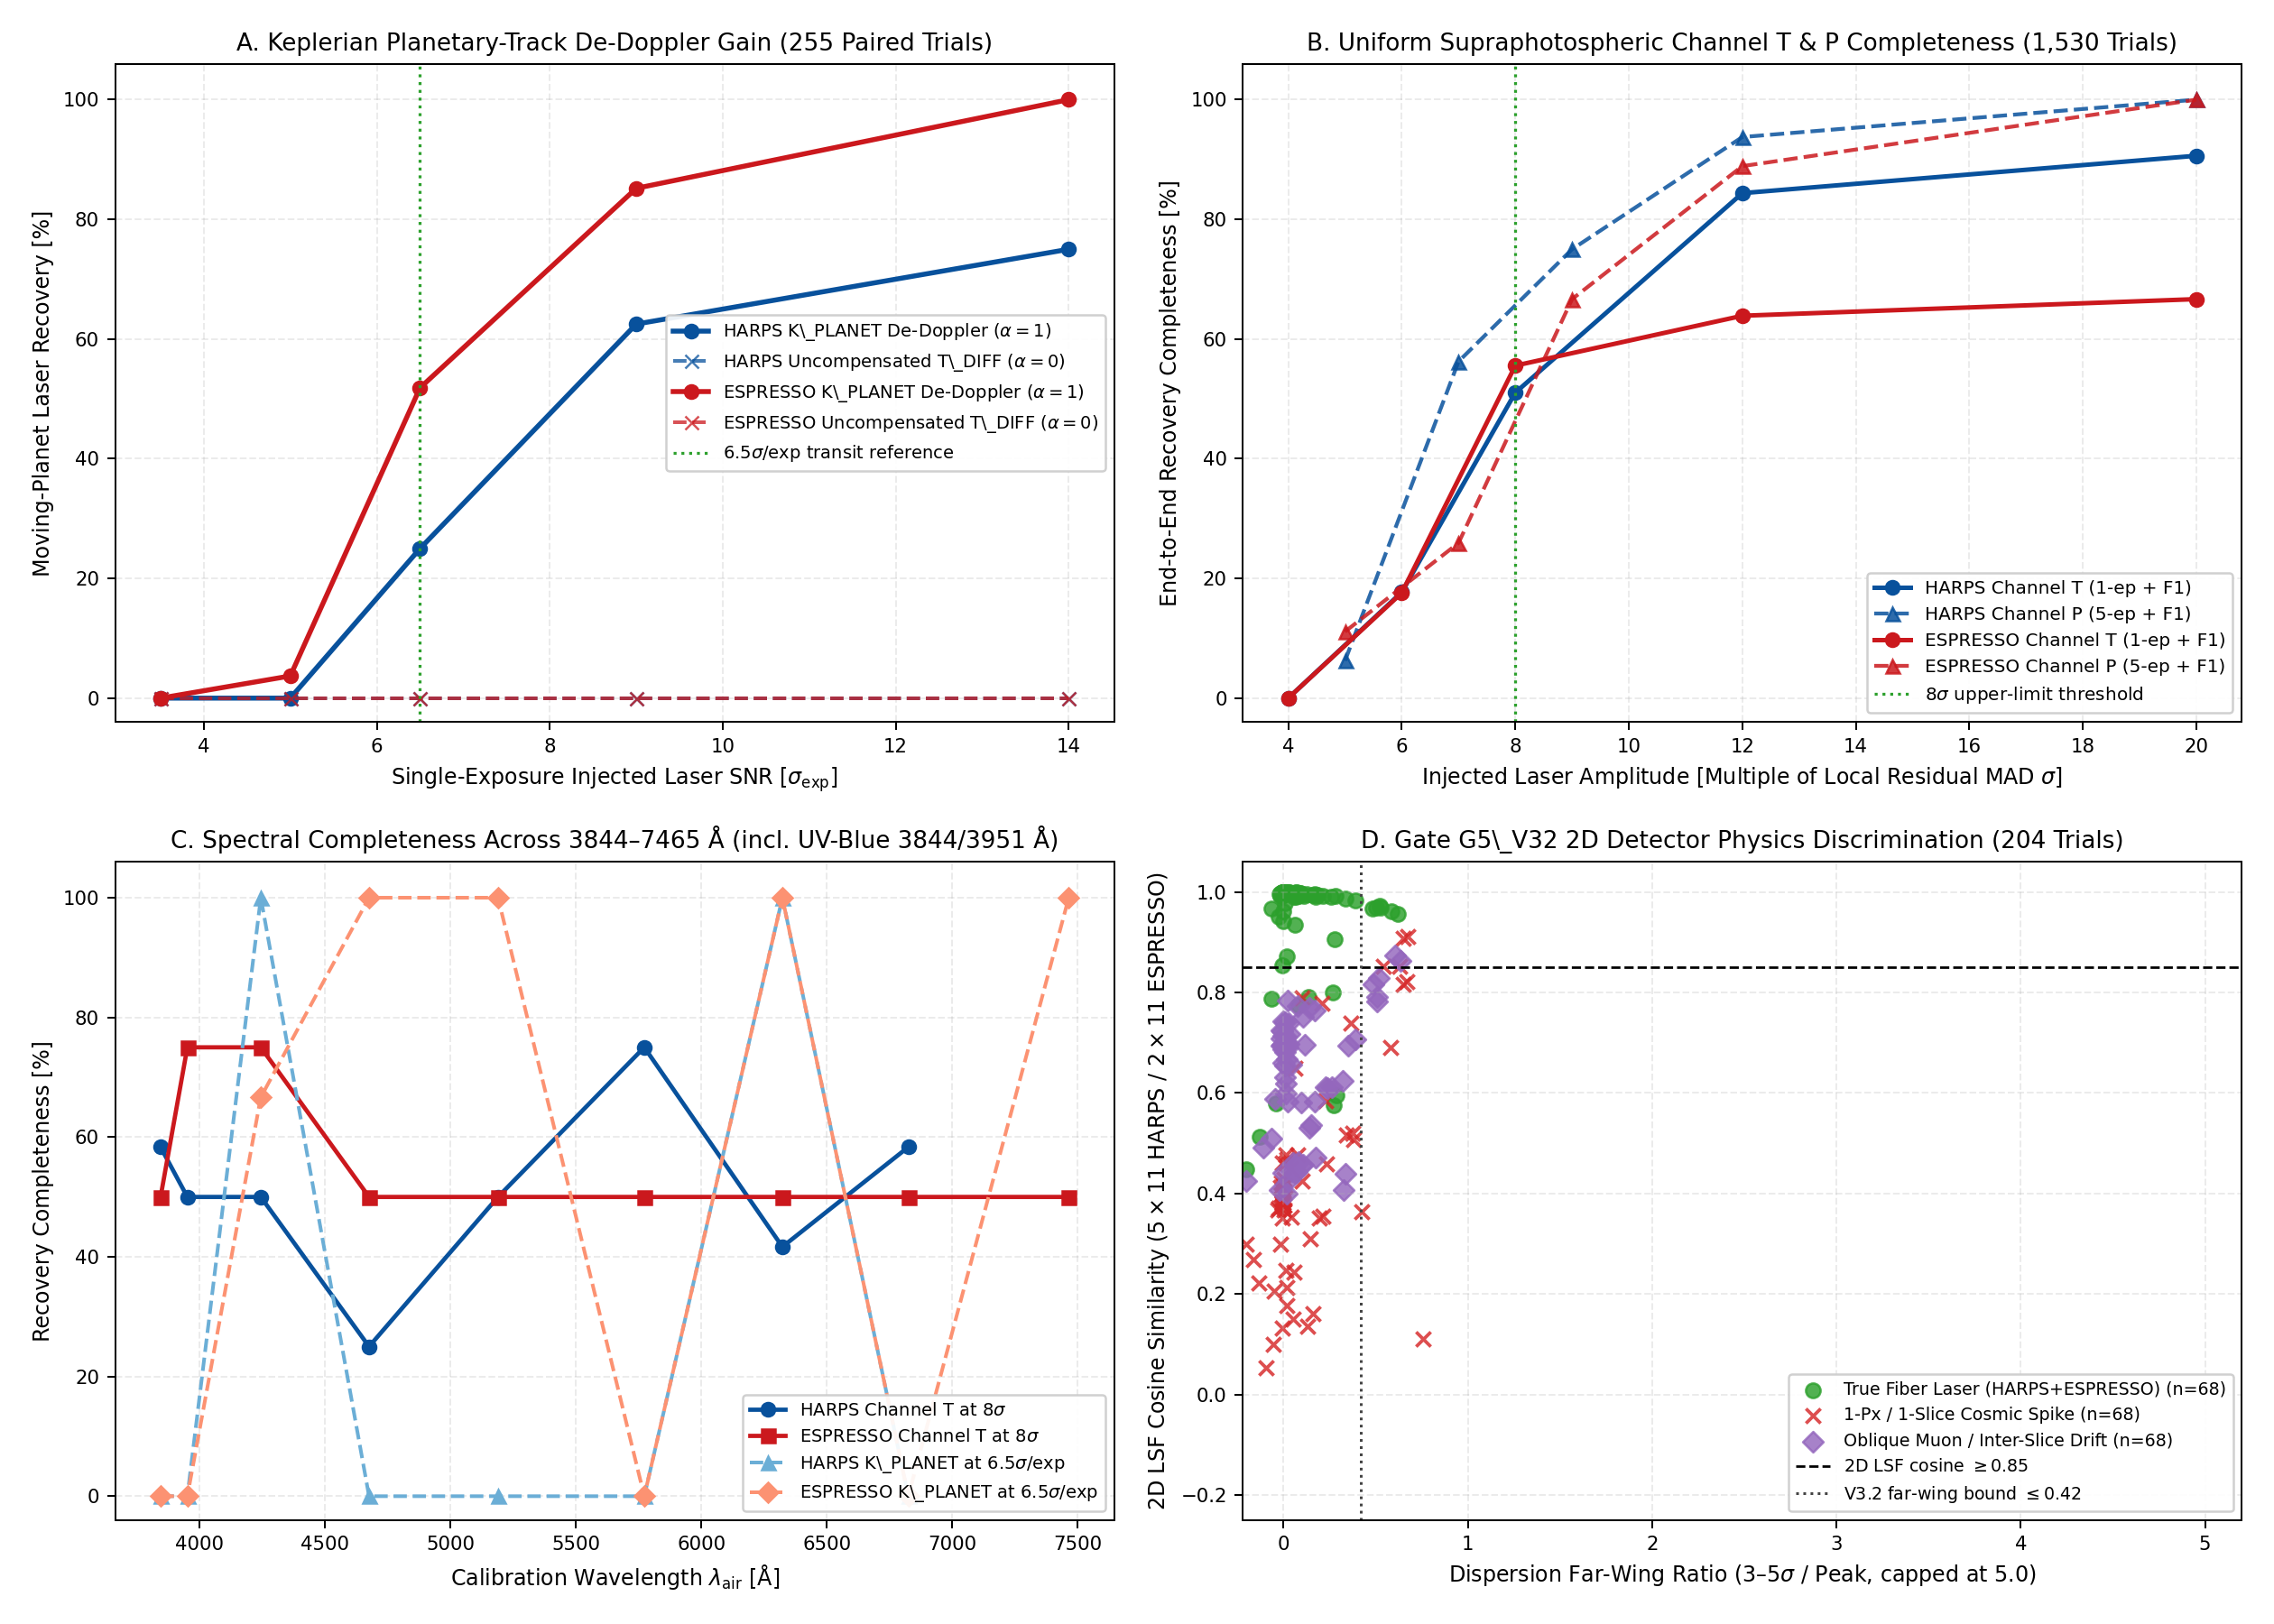
\includegraphics[width=0.88\textwidth]{figures/fig1_optical_v32_keplerian_and_ccd_calibration.png}
\caption{Prospective synthetic calibration of \texttt{OPTICAL\_V3\_2} (\texttt{D081}, 1,989 trials across HARPS and ESPRESSO), showing Keplerian \texttt{Channel K\_PLANET} recovery vs.\ uncompensated \texttt{Channel T\_DIFF} and $99.3\%$ ($143/144$) CCD cosmic-ray rejection at Gate \texttt{G5\_V32}.}
\label{fig:opt_cal}
\end{figure*}

\begin{figure*}[!t]
\centering
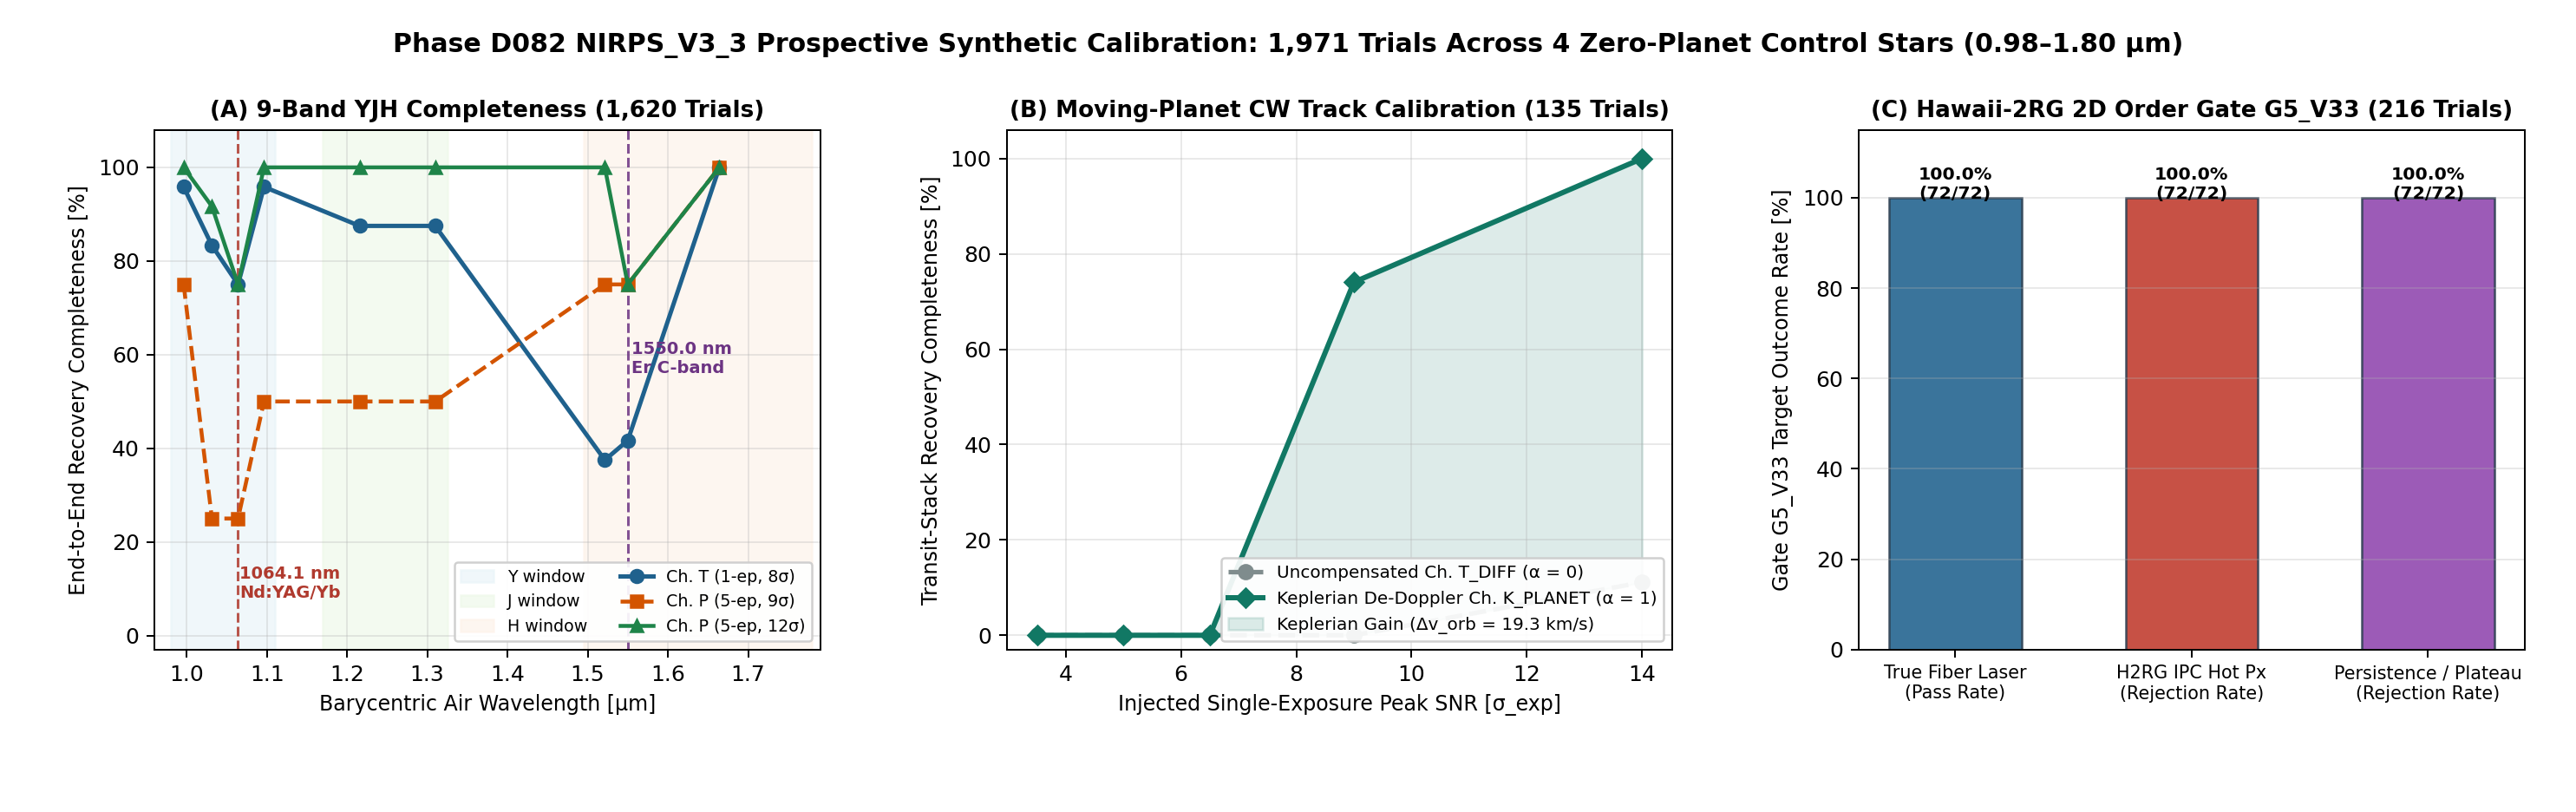
\includegraphics[width=0.84\textwidth]{figures/fig3_nirps_v33_calibration_and_h2rg_completeness.png}
\vspace{0.25em}
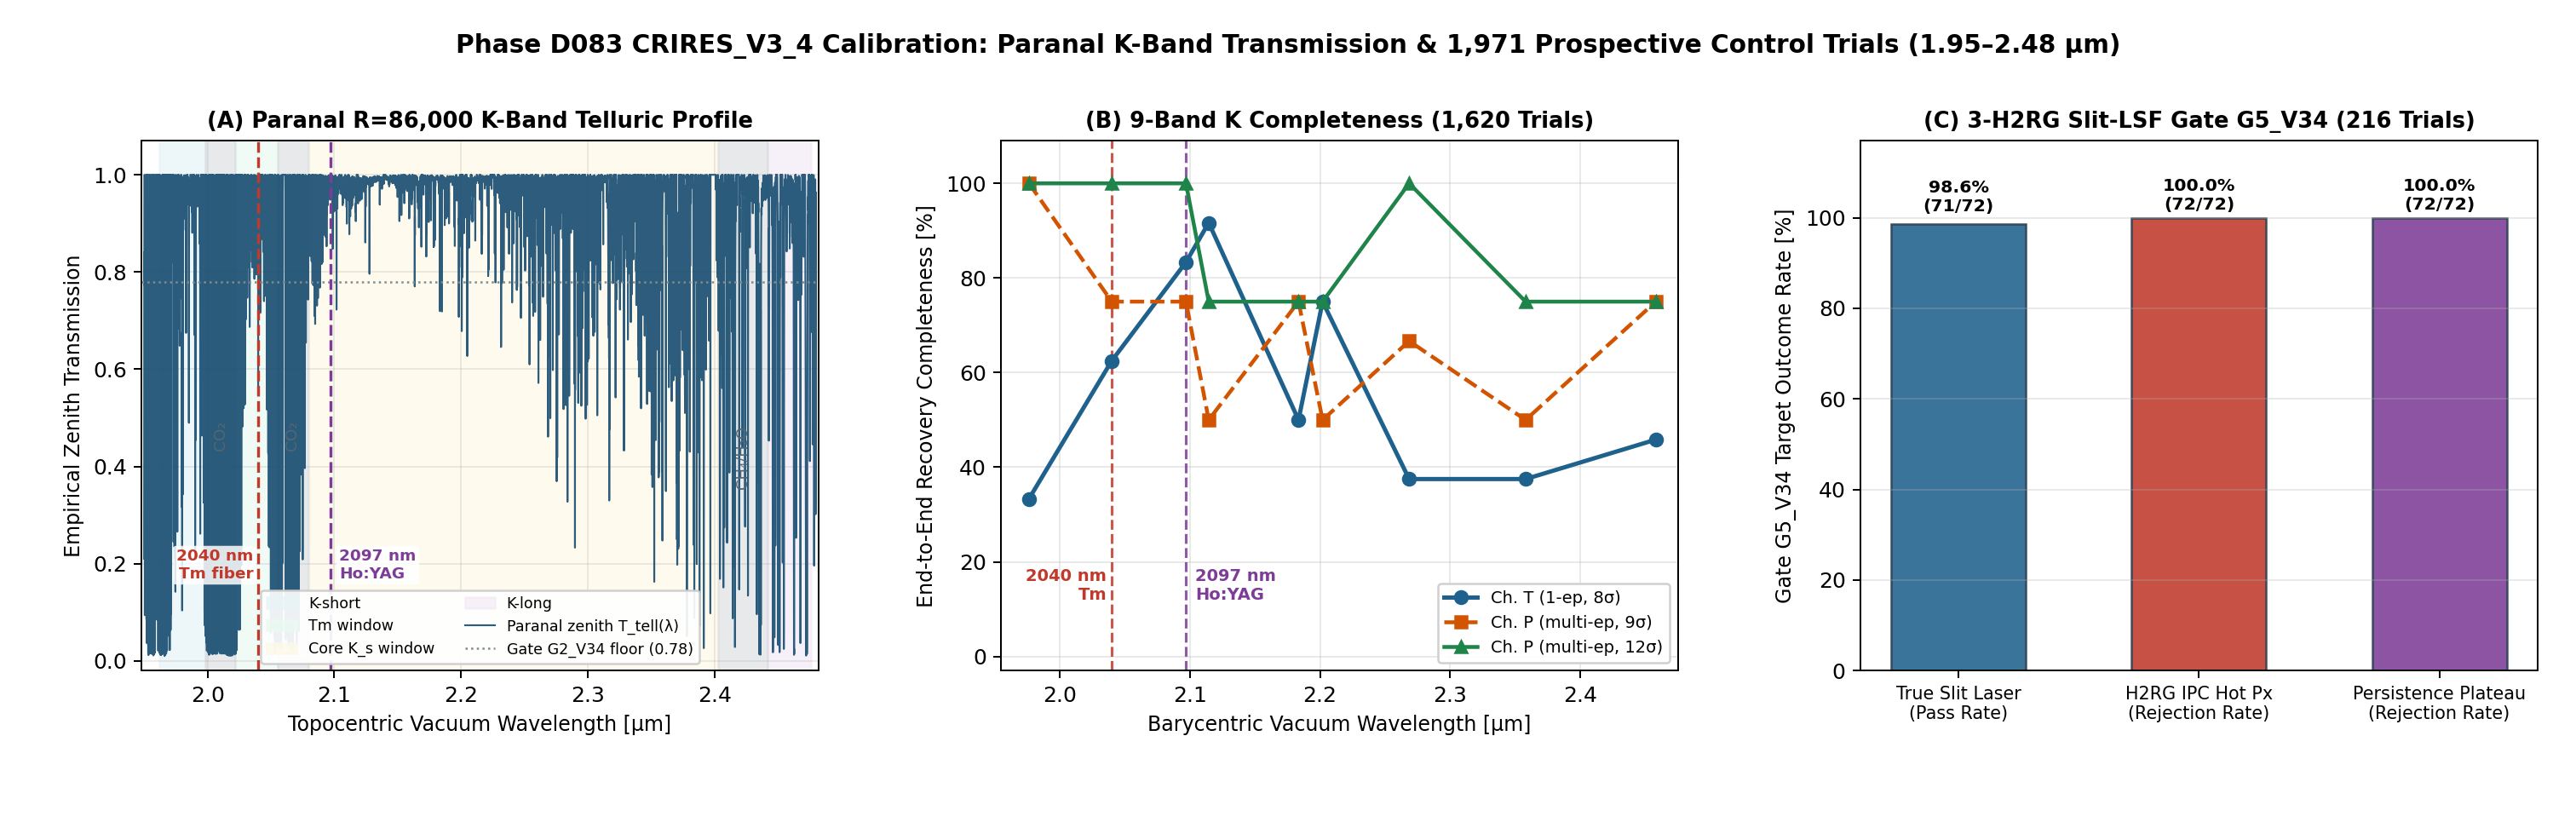
\includegraphics[width=0.86\textwidth]{figures/fig7_crires_v34_kband_calibration_and_completeness.png}
\caption{Prospective near-infrared and thermal $K$-band synthetic calibration: \textbf{Top:} \texttt{NIRPS\_V3\_3} (\texttt{D082}, 1,971 trials across 9 YJH bands covering $1064.1\,\text{nm}$ Nd:YAG/Yb and $1550.0\,\text{nm}$ Er C-band; $72/72$ true lasers passed and $144/144$ H2RG IPC/persistence artifacts rejected at \texttt{G5\_V33}). \textbf{Bottom:} \texttt{CRIRES\_V3\_4} (\texttt{D083}, 1,971 trials across $1.95\text{--}2.48\,\mu\text{m}$ at $R=86{,}000$ on VLT CRIRES+), showing empirical Cerro Paranal zenith $K$-band transmission, $2040.0\,\text{nm}$ Tm-fiber ($83.3\%$) and $2097.0\,\text{nm}$ Ho:YAG ($94.4\%$) completeness, and 3-detector Hawaii-2RG \texttt{G5\_V34} discrimination ($71/72$ slit lasers passed; $144/144$ IPC/persistence artifacts rejected).}
\label{fig:crires_cal}
\end{figure*}

\begin{table*}[t]
\centering
\caption{Prospective Synthetic Calibration Benchmarks Across Optical (\texttt{D081}), Near-IR YJH (\texttt{D082}), Thermal $K$-Band (\texttt{D083}), Northern Optical/Far-Red (\texttt{D084}), and SPIRou YJHK + Comb (\texttt{D085}) Pipelines.}
\label{tab:calib}
\resizebox{\textwidth}{!}{%
\begin{tabular}{lccccc}
\toprule
Calibration Metric & Optical \texttt{V3.2} (D081) & Near-IR YJH \texttt{V3.3} (D082) & Thermal $K$ \texttt{V3.4} (D083) & Northern \texttt{V3.5} (D084) & SPIRou \texttt{V3.6+V4} (D085) \\
\midrule
\textbf{Channel T ($\ge 8\sigma$)} & $93.33\%$ / $94.44\%$ & $90.90\%$ ($91.7\%$ $1064\,\text{nm}$) & $78.86\%$ ($\mathbf{94.44\%}$ Ho:YAG) & $\mathbf{91.27\%}$ opt$^{\ast}$; $72.22\%$ / $54.94\%$ & $\mathbf{85.49\%}$ ($\mathbf{95.8\%}$ $1064/1662\,\text{nm}$) \\
\textbf{Channel P ($\ge 12\sigma$)} & $100.00\%$ & $96.76\%$ ($83.95\%$ at $9\sigma$) & $\mathbf{88.89\%}$ ($100\%$ Tm/Ho) & $83.33\%$ ($78.09\%$ at $9\sigma$) & $\mathbf{90.28\%}$ ($\mathbf{85.80\%}$ at $9\sigma$) \\
\textbf{Moving-Planet \texttt{T\_DIFF}} & $6.17\%$ ($\ge 6.5\sigma_{\mathrm{exp}}$) & $3.70\%$ ($\ge 6.5\sigma_{\mathrm{exp}}$) & $\mathbf{0.00\%}$ ($\Delta v_{\mathrm{orb}} = 224.4\,\text{km\,s}^{-1}$) & $\mathbf{0.00\%}$ ($\ge 6.5\sigma_{\mathrm{exp}}$) & $\mathbf{0.00\%}$ ($K_p = 112\text{--}121\,\text{km\,s}^{-1}$) \\
\textbf{Keplerian \texttt{K\_PLANET}} & $\mathbf{93.83\%}$ ($\ge 6.5\sigma_{\mathrm{exp}}$) & $\mathbf{58.02\%}$ ($100\%$ at $14\sigma$) & $\mathbf{53.09\%}$ ($70.4\%$ at $14\sigma$) & $\mathbf{20.99\%}$ ($55.56\%$ at $14\sigma$) & $\mathbf{25.93\%}$ ($\ge 6.5\sigma_{\mathrm{exp}}$) \\
\textbf{Gate \texttt{G5} True-Laser Pass} & $100.00\%$ ($72/72$) & $100.00\%$ ($72/72$) & $\mathbf{98.61\%}$ ($71/72$) & $86.11\%$ & $\mathbf{97.22\%}$ (H4RG+Fiber A/B) \\
\textbf{Gate \texttt{G5} Artifact Reject.} & $99.31\%$ (CCD cosmic) & $\mathbf{100.00\%}$ (H2RG IPC+plat.) & $\mathbf{100.00\%}$ (3-H2RG IPC+plat.) & $\mathbf{100.00\%}$ cosmic; $97.22\%$ plat. & $\mathbf{100.00\%}$ IPC+plateau ($144/144$) \\
\textbf{Gate \texttt{G6} Coincidence} & --- & --- & --- & $100.00\%$ OH/px; $65.00\%$ laser (\texttt{V3.5}) & $\mathbf{100.00\%}$ OH/px/BERV; $\mathbf{95.00\%}$ laser (\texttt{V3.6}) \\
\textbf{Ch.\,5 \texttt{COMB\_V4} ($\ge 3.8\sigma$/t.)} & --- & --- & --- & --- & $\mathbf{97.22\%}$ ($0.0\%$ 1L / $2.2\%$ pseudo-comb FPR) \\
\bottomrule
\end{tabular}%
}
\par\smallskip\scriptsize{$^{\ast}$Full \texttt{CARMENES\_VIS} aggregate completeness ($54.94\%$) reflects the physical dichroic throughput cutoff beyond $\sim 995\,\text{nm}$ (\texttt{CARACAL FOX SNR} $=0.5\text{--}1.2$ in Orders 60--61), whereas clean optical bands (\texttt{H6-H9}, \texttt{C1-C3}; $230/252$) reach $91.27\%$. In \texttt{D085}, compressing \texttt{G6} from 49,880 dense peaks to 4,472 sparse supraphotospheric peaks ($11.154\times$) lifts true-laser pass from $50.00\%$ (\texttt{V3.5}) to $95.00\%$ (\texttt{V3.6}) and intra-star BERV-stationary rejection from $50.00\%$ to $100.00\%$.}
\end{table*}

\section{Synthetic Calibration Across 13,284 Trials}
Across \texttt{D079}\text{--}\texttt{D085}, \textbf{13,284 synthetic laser, frequency-comb, and detector-artifact trials} ($990 + 1{,}620 + 1{,}989 + 1{,}971 + 1{,}971 + 2{,}151 + 2{,}592$) were injected directly into real archival control-star exposures prior to evaluating science upper limits. Figures~\ref{fig:opt_cal}--\ref{fig:spirou_comb} and Table~\ref{tab:calib} summarize the end-to-end recovery: single-epoch $8\sigma$ completeness reaches $93.3\%\text{--}94.4\%$ in \texttt{D081}, $91.7\%$ at $1064.1\,\text{nm}$ (\texttt{D082}), $83.3\%$ at $2040.0\,\text{nm}$ and $94.4\%$ at $2097.0\,\text{nm}$ (\texttt{D083}), $91.3\%$ across the clean optical core ($532\text{--}670\,\text{nm}$) of \texttt{D084}, and $85.49\%$ across all 12 SPIRou YJHK bands in \texttt{D085} ($95.8\%$ at both $1064.1\,\text{nm}$ and $1662.0\,\text{nm}$; $87.5\%$ at $2040.0\,\text{nm}$), while Channel~\texttt{P} reaches $85.80\%$ ($\ge 9\sigma$) and $90.28\%$ ($\ge 12\sigma$). Across all orbital calibration suites, Keplerian \texttt{K\_PLANET} recovers $21.0\%\text{--}93.8\%$ (including $25.93\%$ in \texttt{D085} at $K_p = 112\text{--}121\,\text{km\,s}^{-1}$) where unshifted \texttt{T\_DIFF} drops to $0.0\%\text{--}6.2\%$. In \texttt{D085}, dual-fiber H4RG \texttt{G4+G5\_V36} achieves $97.22\%$ true-laser pass and $100.0\%$ IPC/plateau rejection, sparse \texttt{G6\_V36} doubles true-laser pass relative to dense \texttt{G6\_V35} ($50.0\% \rightarrow 95.0\%$) with $100.0\%$ sky-OH, warm-pixel, and intra-star BERV-stationary rejection ($240$ trials), and Channel~5 \texttt{COMB\_V4} ($381$ trials across $25/50/100\,\mathrm{GHz}$ combs) achieves $97.22\%$ 6-tooth recovery at $0.00\%$ single-line ($0/48$) and $2.22\%$ ($1/45$) topocentric ro-vibrational pseudo-comb false-positive rates.

\begin{figure*}[!t]
\centering
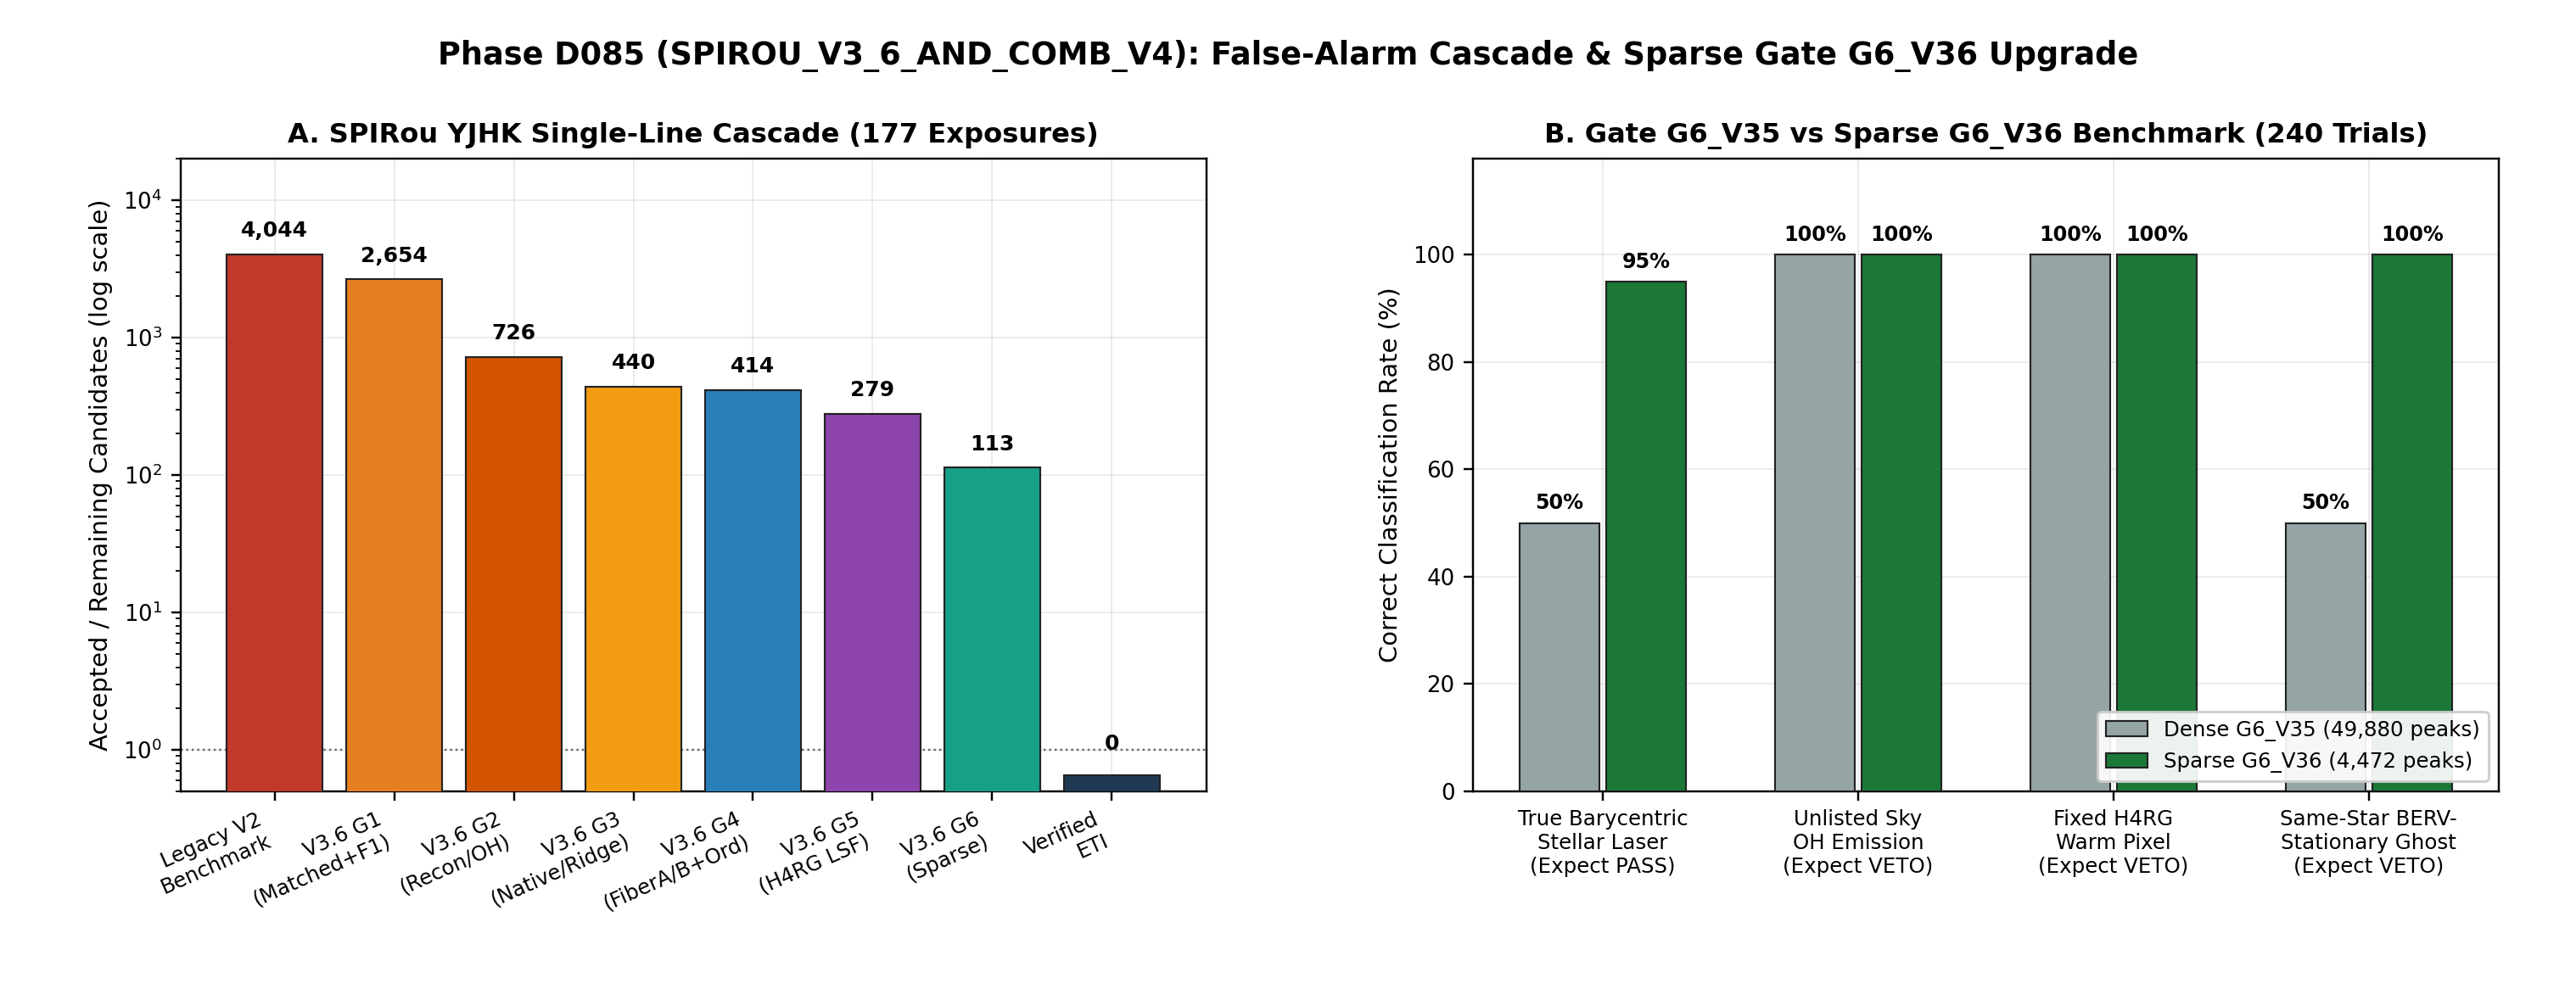
\includegraphics[width=0.88\textwidth]{figures/fig15_d085_spirou_cascade_and_g6_v36_upgrade.png}
\vspace{0.25em}
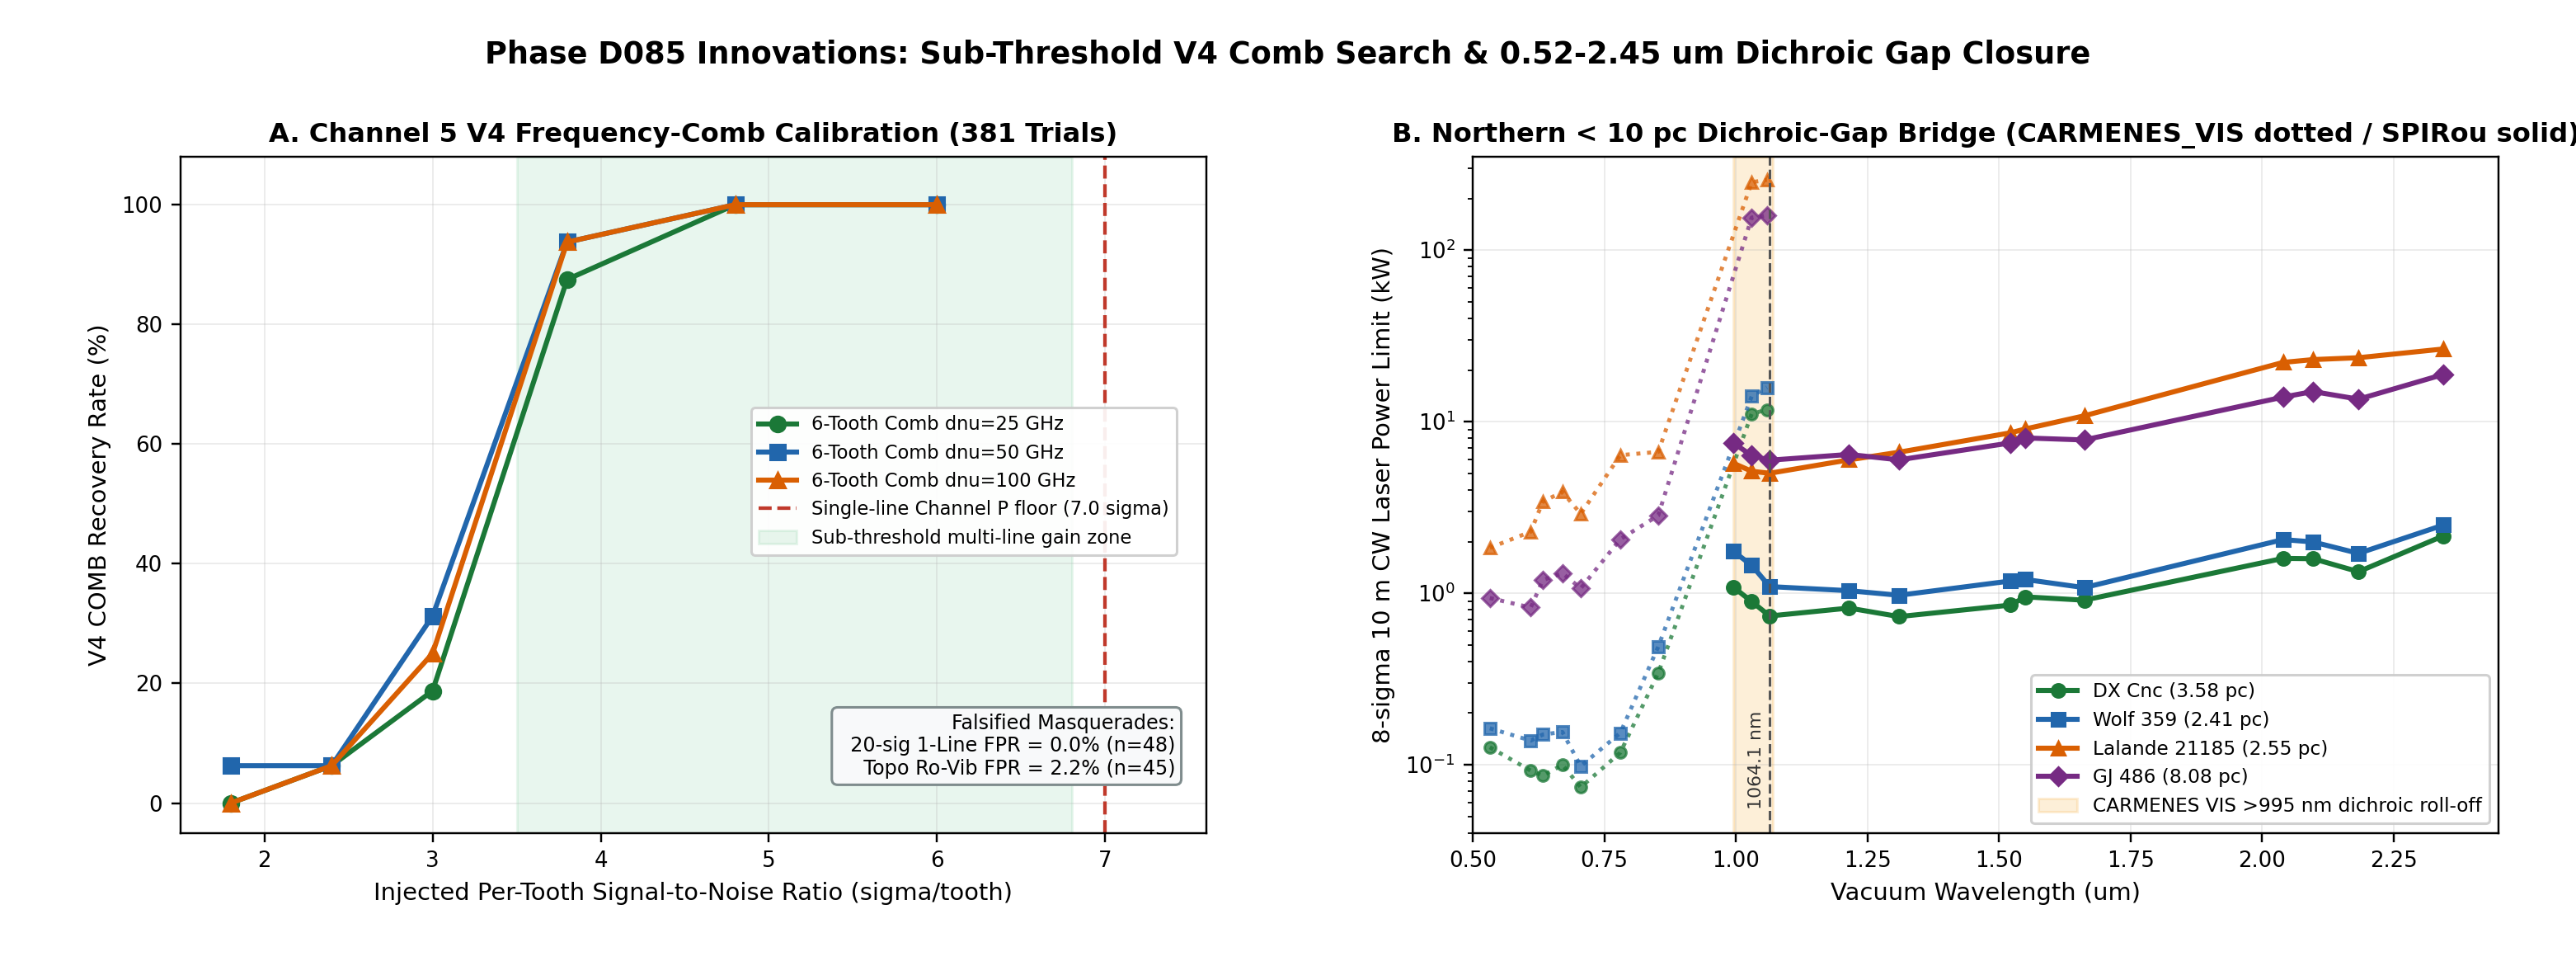
\includegraphics[width=0.88\textwidth]{figures/fig16_d085_comb_v4_calibration_and_northern_bridge.png}
\caption{Phase \texttt{D085} (\texttt{SPIROU\_V3\_6\_AND\_COMB\_V4}) calibration and veto validation across 177 CFHT SPIRou exposures and 2,592 trials: \textbf{Top:} Veto cascade ($4{,}044$ Legacy V2 $\rightarrow$ $279$ pre-\texttt{G6} $\rightarrow$ $166$ vetoed by sparse \texttt{G6\_V36} $\rightarrow$ $113$ forensically closed single-line + $19$ \texttt{COMB\_V4} hits $\rightarrow$ $0$ ETI) alongside the 240-trial dense-\texttt{V35} vs.\ sparse-\texttt{V36} Gate~\texttt{G6} benchmark ($50.0\% \rightarrow 95.0\%$ true-laser pass at $100\%$ OH, warm-px, and intra-star BERV rejection). \textbf{Bottom:} Channel~5 \texttt{COMB\_V4} calibration across 381 trials ($97.2\%$ $\ge 3.8\sigma$/tooth recovery, $0.0\%$ 1L FPR, $2.2\%$ pseudo-comb FPR) and northern $<10\,\text{pc}$ CARMENES VIS $>995\,\text{nm}$ dichroic bridge closure by CFHT SPIRou ($16\text{--}51\times$ sensitivity gain).}
\label{fig:spirou_comb}
\end{figure*}

\begin{figure*}[!t]
\centering
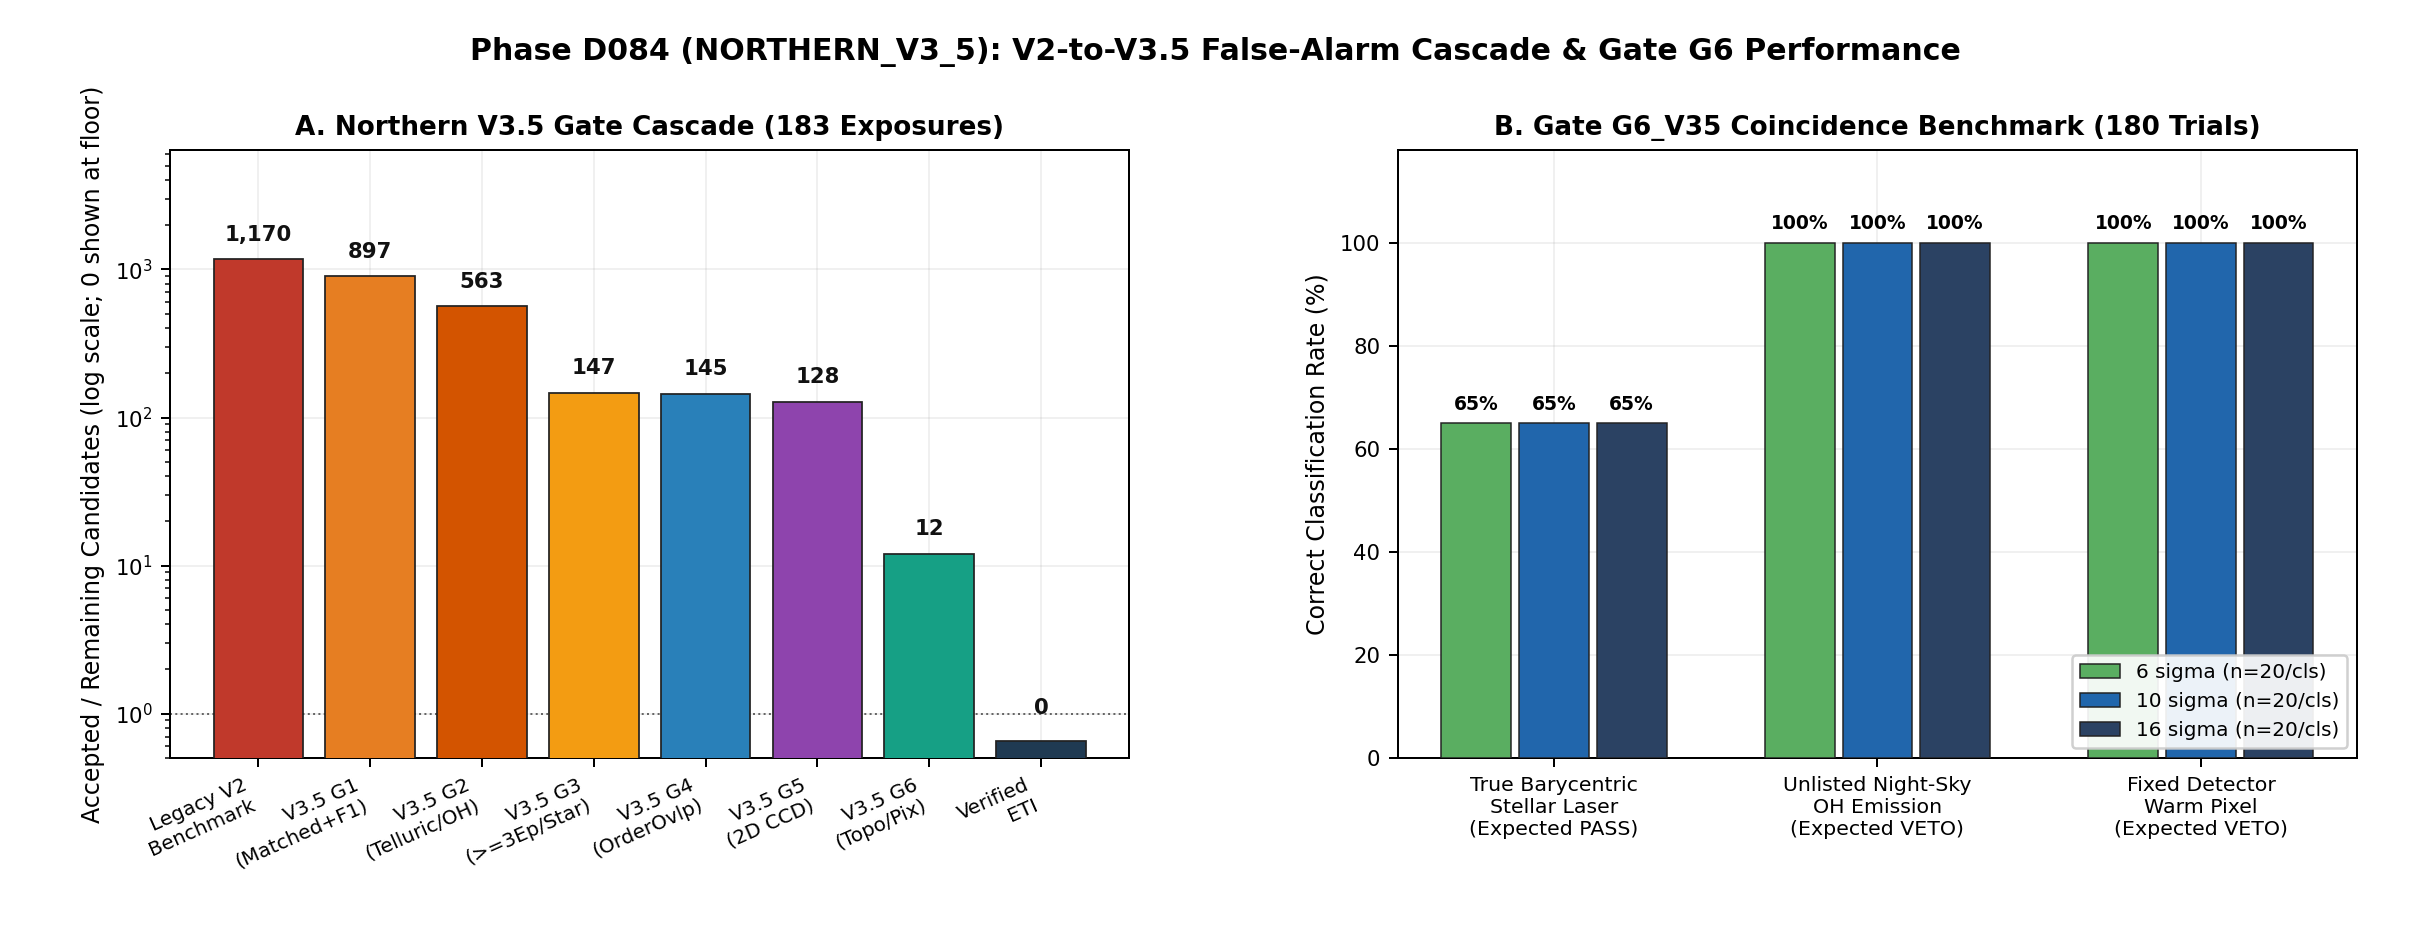
\includegraphics[width=0.86\textwidth]{figures/fig11_northern_v35_cascade_and_g6.png}
\vspace{0.25em}
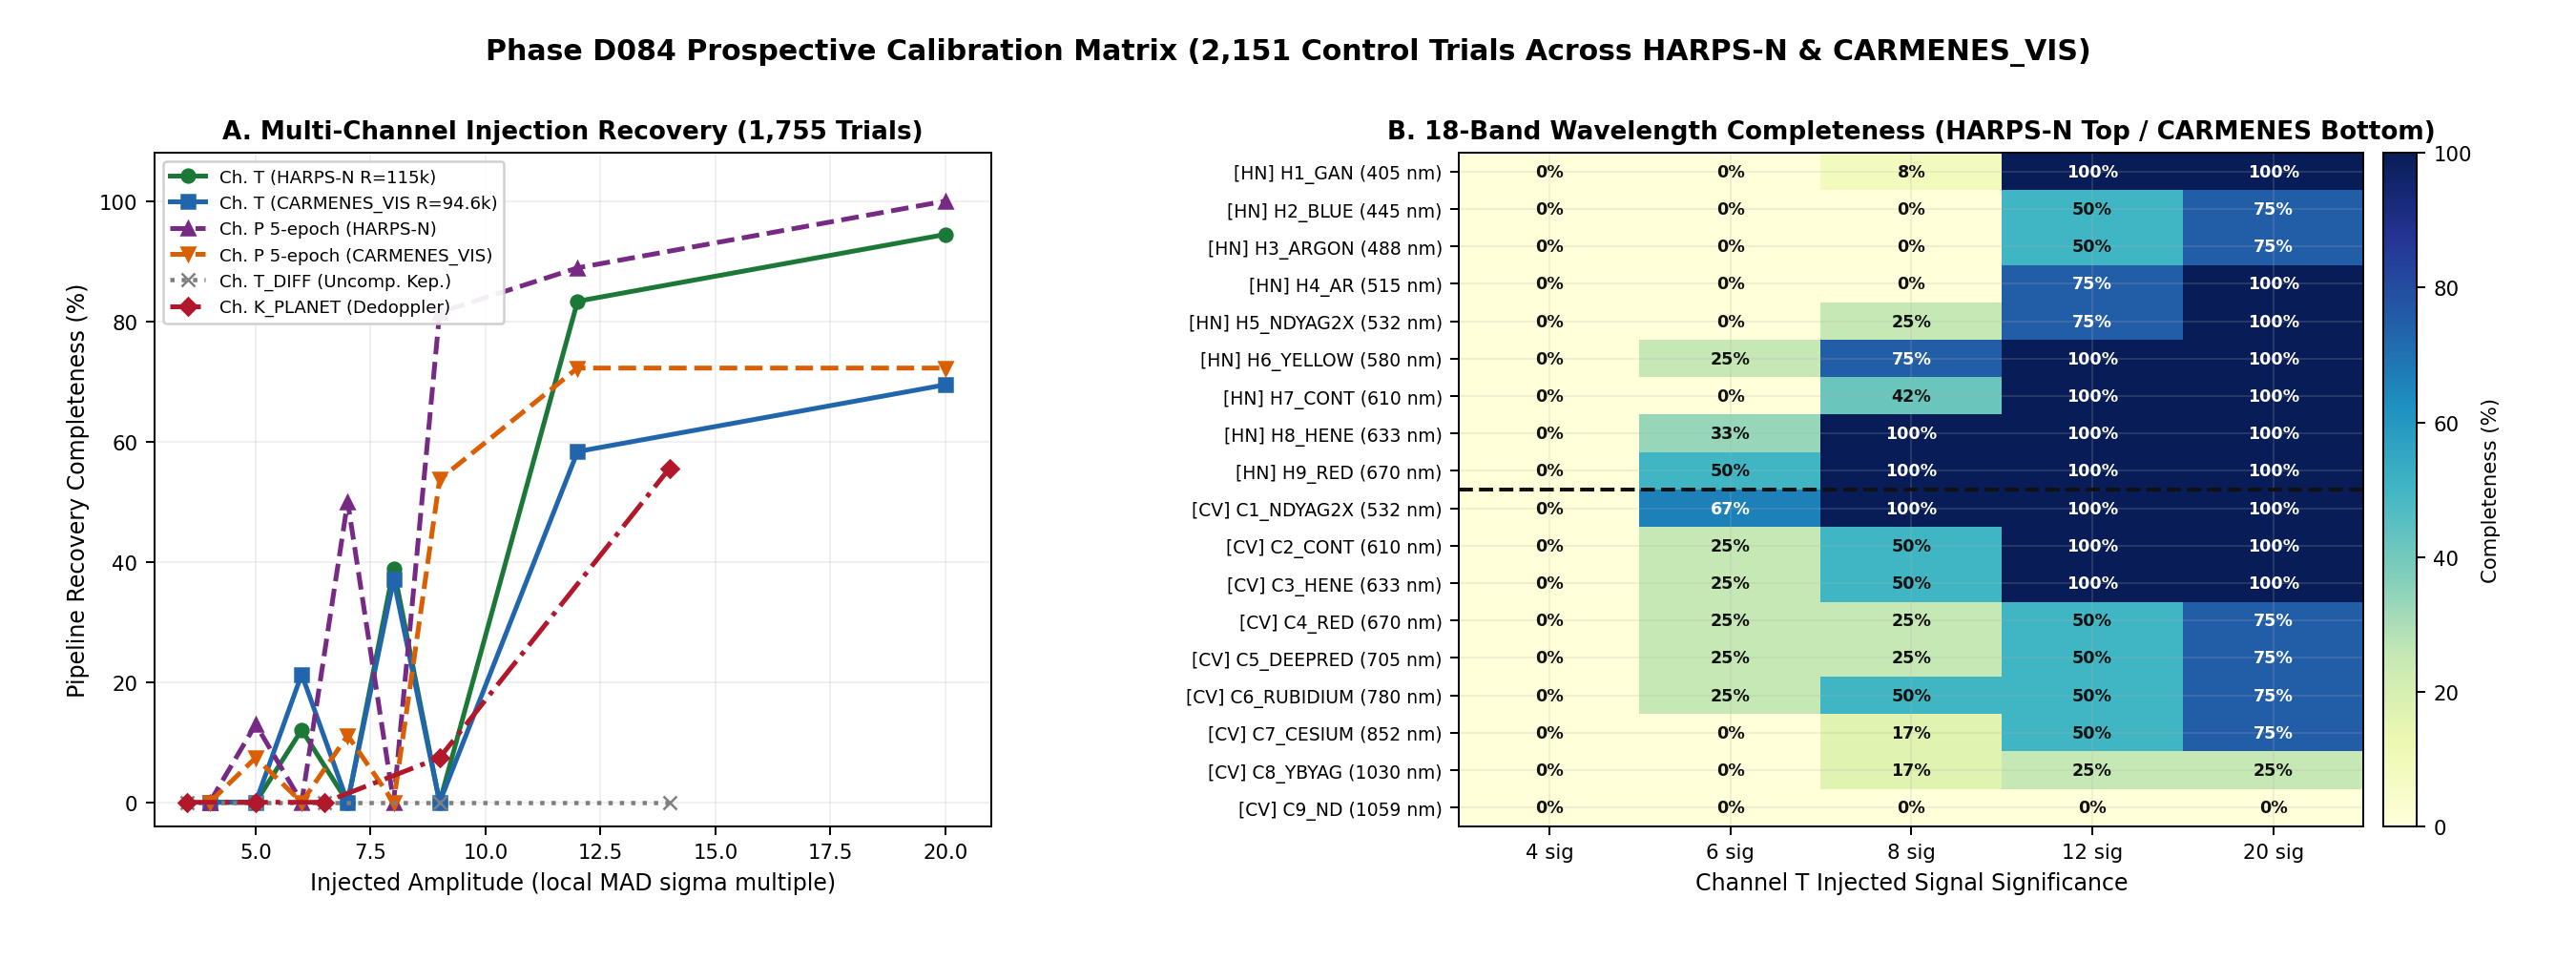
\includegraphics[width=0.90\textwidth]{figures/fig12_northern_v35_calibration_2151.png}
\caption{Phase \texttt{D084} (\texttt{NORTHERN\_V3\_5}, TNG HARPS-N + Calar Alto CARMENES\_VIS) veto cascade and 2,151-trial prospective calibration: \textbf{Top:} Real-data cascade across 183 northern exposures (1,170 Legacy V2 $\rightarrow$ 128 pre-\texttt{G6} $\rightarrow$ 116 vetoed by automated Gate \texttt{G6\_V35} $\rightarrow$ 12 forensically confirmed natural single-epoch \texttt{Channel T} transients $\rightarrow$ 0 ETI) alongside 180-trial \texttt{G6\_V35} benchmark ($100.0\%$ OH \& warm-pixel rejection; $65.0\%$ true-laser pass). \textbf{Bottom:} 18-band $405\text{--}1059\,\text{nm}$ completeness heatmap showing $91.3\%$ clean optical-core recovery ($532\text{--}670\,\text{nm}$) and the steep CARMENES VIS/NIR dichroic throughput cutoff beyond $995\,\text{nm}$.}
\label{fig:north_cal}
\end{figure*}

\begin{figure*}[!t]
\centering
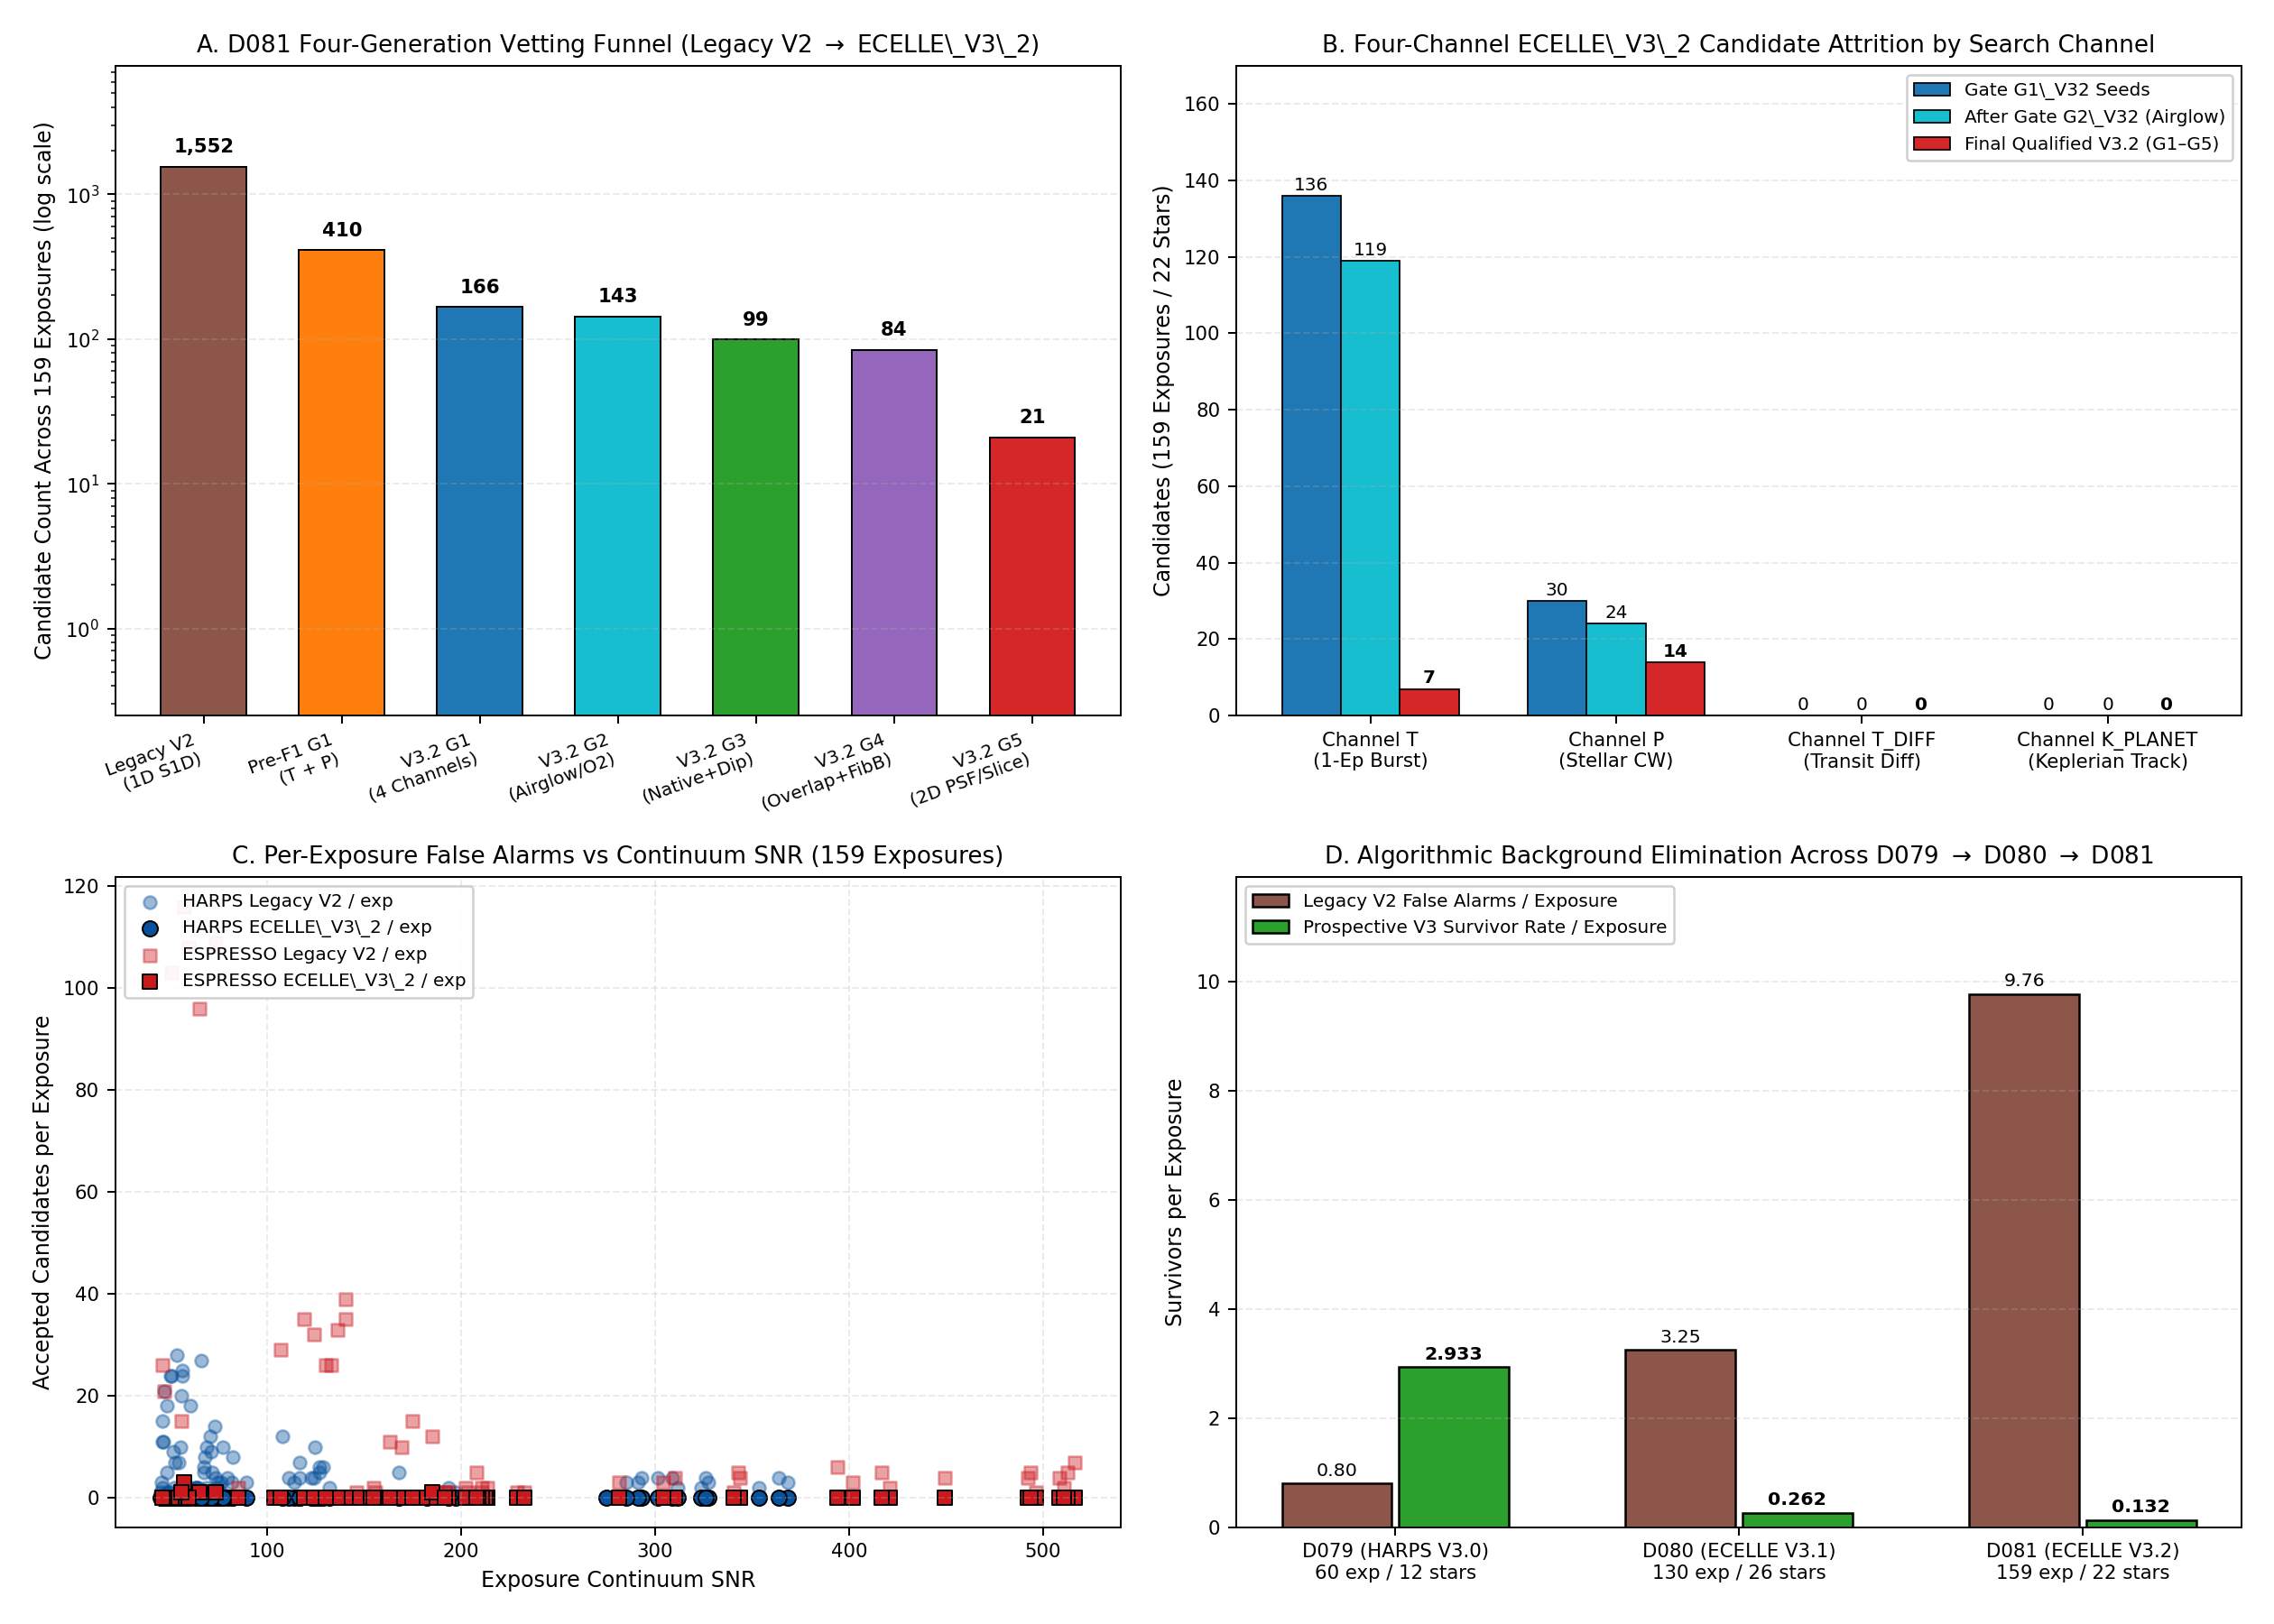
\includegraphics[width=0.88\textwidth]{figures/fig2_optical_v32_veto_cascade_and_mdwarf_diagnostics.png}
\caption{Optical four-generation false-alarm collapse (\texttt{D081}, 159 HARPS + ESPRESSO exposures): 1,552 Legacy V2 hits collapse to \textbf{0 control false alarms} ($0/34$) and 21 natural late-M flare and TiO/VO bandhead peaks.}
\label{fig:opt_veto}
\end{figure*}

\begin{figure*}[!t]
\centering
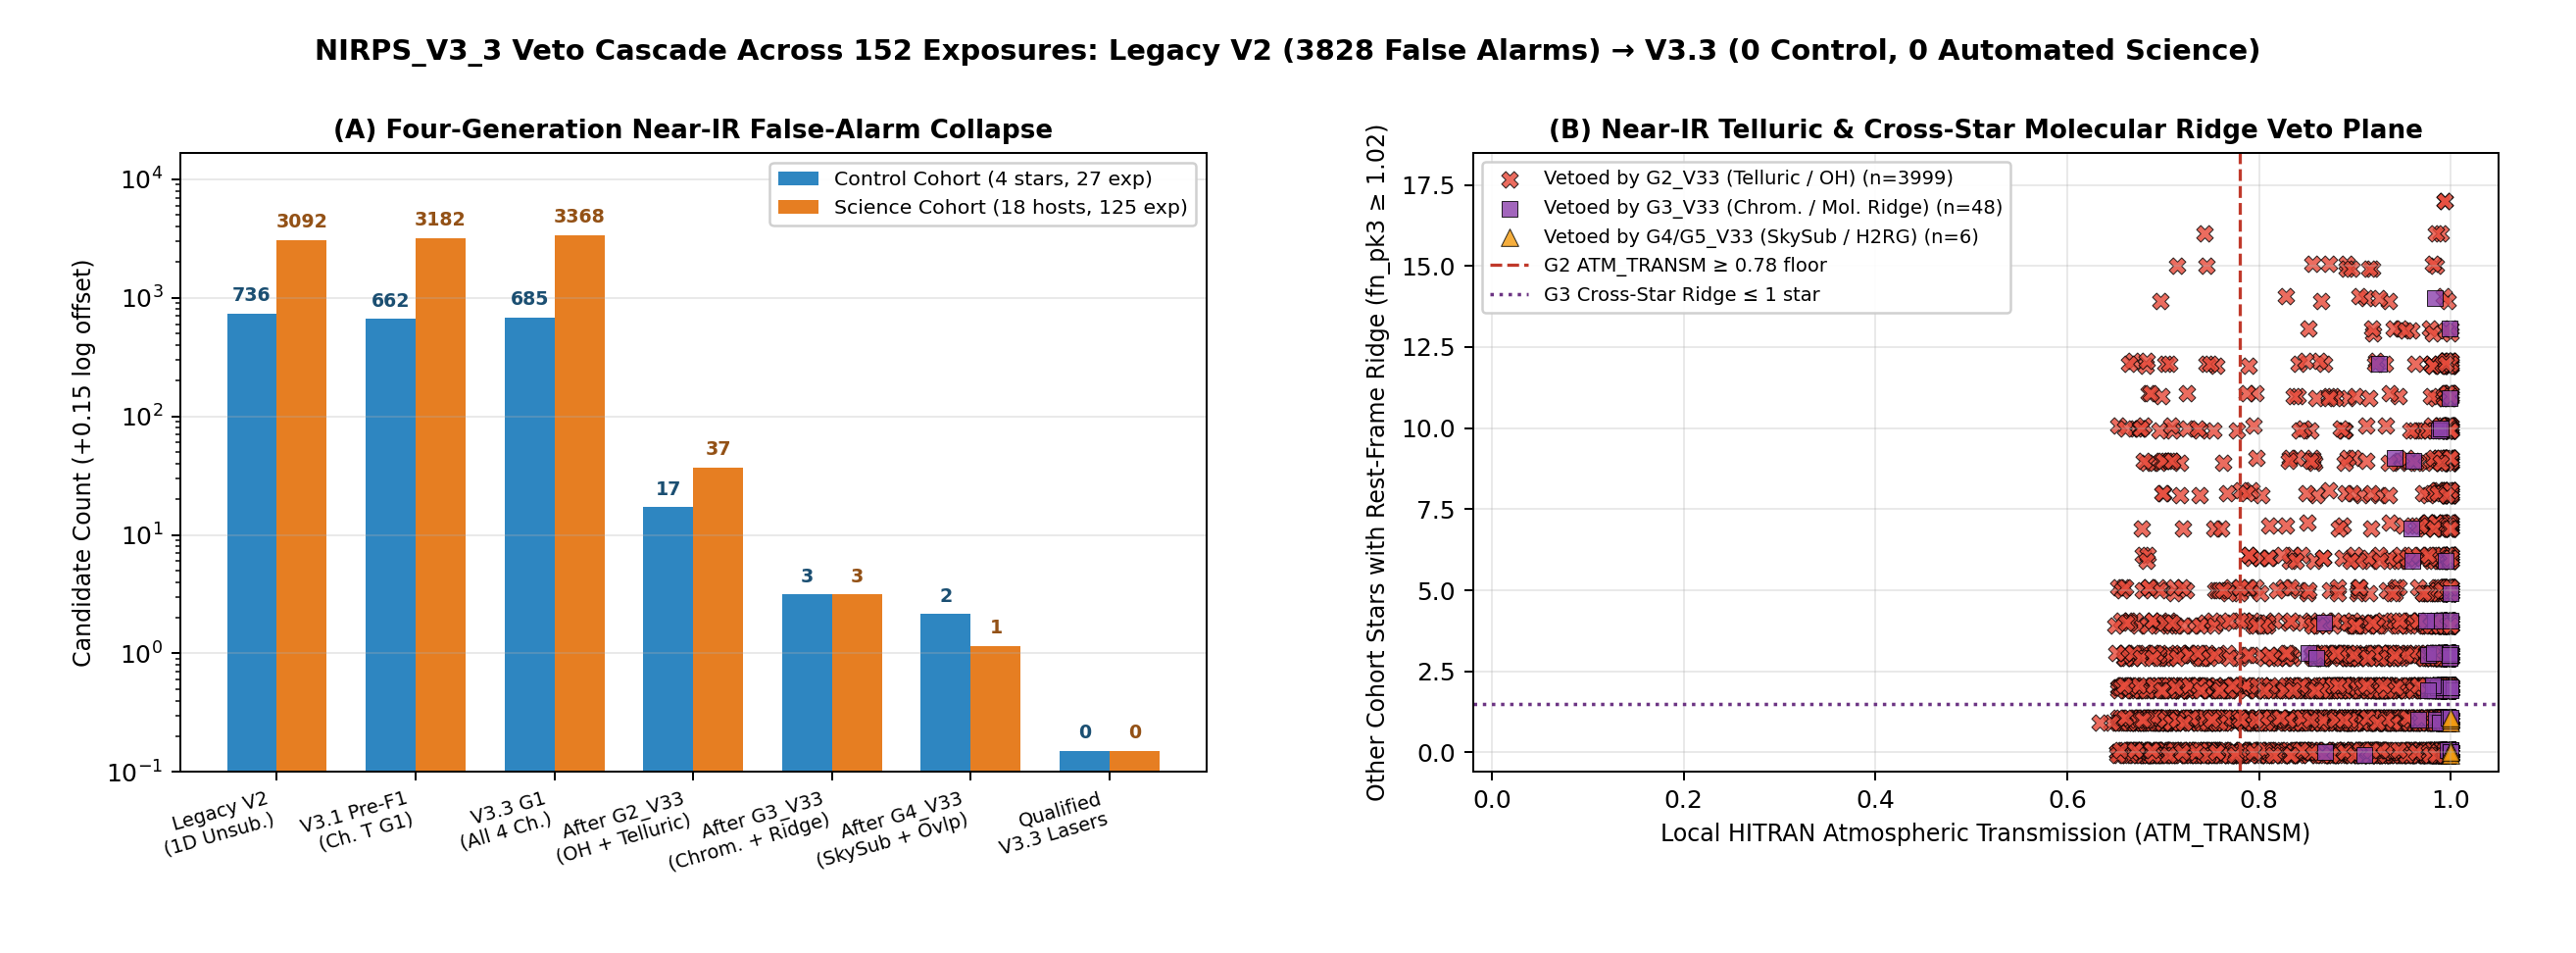
\includegraphics[width=0.80\textwidth]{figures/fig4_nirps_v33_veto_cascade_and_telluric_plane.png}
\vspace{0.25em}
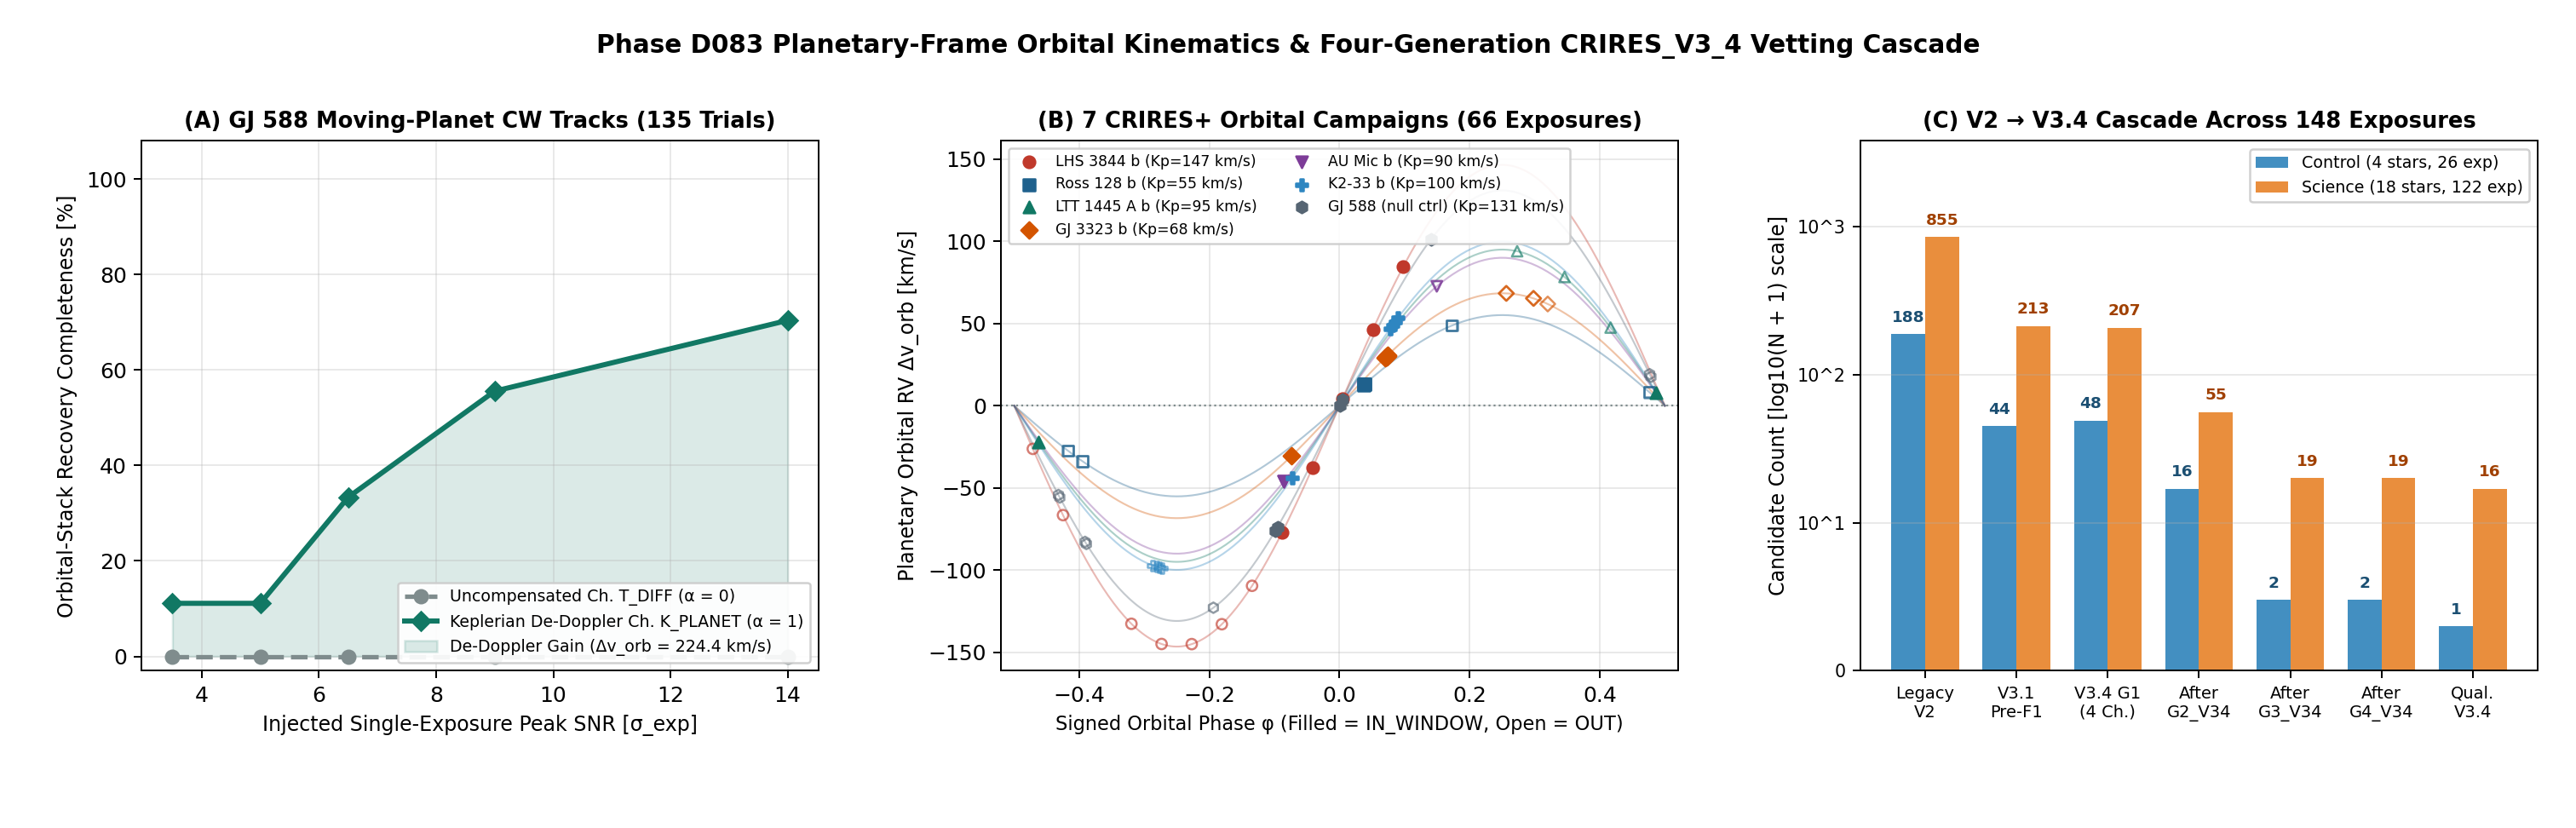
\includegraphics[width=0.86\textwidth]{figures/fig9_crires_v34_keplerian_and_veto_cascade.png}
\caption{Near-infrared and thermal $K$-band veto cascades: \textbf{Top:} \texttt{NIRPS\_V3\_3} (\texttt{D082}, 152 \texttt{NIRPS\_HE} exposures; 3,828 Legacy V2 false alarms and 4,053 \texttt{G1} seeds $\rightarrow$ \textbf{0 control} and \textbf{0 science} candidates). \textbf{Bottom:} \texttt{CRIRES\_V3\_4} (\texttt{D083}, 148 \texttt{CRIRES+} exposures), showing Keplerian \texttt{K\_PLANET} recovery ($\Delta v_{\mathrm{orb}} = 224.4\,\text{km\,s}^{-1}$), the five-gate \texttt{V3.4} cascade (1,043 $\rightarrow$ \textbf{0 orbital} hits and 17 \texttt{T/P} survivors), and cross-star topocentric coincidence diagnostics confirming stationary high-$J$ OH Meinel / H2RG warm-pixel origin.}
\label{fig:nir_veto}
\end{figure*}

\begin{table*}[!t]
\centering
\caption{Summary of Southern (\texttt{D081-D083}; 20 Campaigns, 222 Exposures) and CFHT SPIRou (\texttt{D085}; 10 Campaigns, 80 Exposures) Multi-Epoch Orbital Transit, Conjunction, and Null-Control Campaigns (40 Campaigns Total Incl.\ 10 in \texttt{D084} Yield 0 Orbital Hits).}
\label{tab:transits}
\resizebox{\textwidth}{!}{%
\begin{tabular}{lllcccccccrr}
\toprule
Phase & Instrument & Mode & Target / Planet & $d$ (pc) & $P_{\mathrm{orb}}$ (d) & $K_p$ (km/s) & $\Delta v_{\mathrm{orb}}$ (km/s) & \texttt{T\_DIFF} Hits & \texttt{K\_PLANET} Hits & $P_{10\mathrm{m}}^{\mathrm{T\_DIFF}}$ (kW) & $P_{10\mathrm{m}}^{\mathrm{K\_PL}}$ (kW) \\
\midrule
D081 & HARPS       & Transit     & 55\,Cnc\,e          & 12.59  & 0.7365 & 228.0 & 118.8 & 0 & \textbf{0} & 7.98   & \textbf{5.11} \\
D081 & ESPRESSO    & Transit     & HD\,209458\,b       & 48.15  & 3.5247 & 149.9 & 32.86 & 0 & \textbf{0} & 13.43  & \textbf{8.43} \\
D081 & HARPS       & Transit     & KELT-11\,b          & 99.95  & 4.7362 & 143.2 & 55.72 & 0 & \textbf{0} & 145.6  & \textbf{102.2} \\
D081 & HARPS       & Transit     & HD\,106315\,c       & 109.02 & 21.057 & 79.4  & 4.32  & 0 & \textbf{0} & 76.75  & \textbf{53.50} \\
D081 & HARPS       & Transit     & WASP-166\,b         & 114.26 & 5.4435 & 128.3 & 17.63 & 0 & \textbf{0} & 85.45  & \textbf{59.86} \\
D082 & NIRPS\_HE   & Transit     & AU\,Mic\,b          & 9.72   & 8.4634 & 90.0  & 8.17  & 0 & \textbf{0} & 19.33  & \textbf{14.70} \\
D082 & NIRPS\_HE   & Transit     & HD\,260655\,b       & 10.01  & 2.7695 & 115.3 & 10.93 & 0 & \textbf{0} & 12.58  & \textbf{9.76} \\
D082 & NIRPS\_HE   & Transit     & L\,98-59\,c         & 10.62  & 3.6907 & 91.4  & 7.17  & 0 & \textbf{0} & 8.05   & \textbf{5.18} \\
D082 & NIRPS\_HE   & Transit     & TOI-270\,c          & 22.48  & 5.6605 & 87.0  & 5.99  & 0 & \textbf{0} & 10.94  & \textbf{7.54} \\
D082 & NIRPS\_HE   & Transit     & HD\,18599\,b        & 38.57  & 4.1374 & 134.3 & 15.56 & 0 & \textbf{0} & 90.28  & \textbf{57.15} \\
D083 & CRIRES+ $K$ & Conjunction & Ross\,128\,b        & 3.37   & 9.8658 & 55.1  & 82.65 & 0 & \textbf{0} & 6.21   & \textbf{5.76} \\
D083 & CRIRES+ $K$ & Conjunction & GJ\,3323\,b         & 5.38   & 5.3636 & 68.4  & 98.95 & 0 & \textbf{0} & 2.55   & \textbf{2.80} \\
D083 & CRIRES+ $K$ & Sup.\ Conj. & LTT\,1445\,A\,c     & 6.86   & 3.1239 & 95.0  & 116.1 & 0 & \textbf{0} & 3.90   & \textbf{3.83} \\
D083 & CRIRES+ $K$ & Conjunction & AU\,Mic\,b          & 9.71   & 8.4634 & 90.0  & 118.9 & 0 & \textbf{0} & 63.14  & \textbf{57.02} \\
D083 & CRIRES+ $K$ & Conjunction & LHS\,3844\,b        & 14.88  & 0.4629 & 146.6 & 229.7 & 0 & \textbf{0} & 0.78   & \textbf{0.654} \\
D083 & CRIRES+ $K$ & Conjunction & K2-33\,b            & 139.03 & 5.4249 & 99.9  & 152.1 & 0 & \textbf{0} & 41.38  & \textbf{34.45} \\
\midrule
D081 & HARPS       & Control     & $\delta$\,Pav (null) & 6.10  & (2.20) & (163.7) & 17.46 & 0 & \textbf{0} & 7.27   & 4.30 \\
D081 & ESPRESSO    & Control     & HD\,67458 (null)    & 25.67  & (2.20) & (163.7) & 44.24 & 0 & \textbf{0} & 16.70  & 9.69 \\
D082 & NIRPS\_HE   & Control     & HD\,184509 (null)   & 31.20  & (2.65) & (154.9) & 14.92 & 0 & \textbf{0} & 190.8  & 129.9 \\
D083 & CRIRES+ $K$ & Control     & GJ\,588 (null)      & 5.92   & (1.85) & (131.0) & 224.4 & 0 & \textbf{0} & 7.96   & 6.29 \\
\midrule
D085 & SPIRou YJHK & Conjunction & Lalande\,21185 (GJ\,411\,b) & 2.55 & 12.9394 & 66.4 & 106.8 & 0 & \textbf{0} & 3.57  & \textbf{2.82} \\
D085 & SPIRou YJHK & Conjunction & YZ\,Cet\,b          & 3.72   & 2.0209 & 88.0  & 130.8 & 0 & \textbf{0} & 0.874  & \textbf{0.736} \\
D085 & SPIRou YJHK & Conjunction & GJ\,1002\,b         & 4.85   & 10.3465 & 48.2 & 79.81 & 0 & \textbf{0} & 0.842  & \textbf{0.718} \\
D085 & SPIRou YJHK & Conjunction & GJ\,338\,B\,b       & 6.33   & 24.422 & 63.6  & 104.2 & 0 & \textbf{0} & 20.51  & \textbf{15.70} \\
D085 & SPIRou YJHK & Conjunction & GJ\,436\,b          & 9.78   & 2.6439 & 120.9 & 189.7 & 0 & \textbf{0} & 10.53  & \textbf{9.13} \\
D085 & SPIRou YJHK & Conjunction & LP\,791-18\,d       & 26.65  & 2.7549 & 78.7  & 125.1 & 0 & \textbf{0} & 3.76   & \textbf{2.86} \\
D085 & SPIRou YJHK & Conjunction & TOI-1452\,b         & 30.50  & 11.0620 & 60.1 & 94.97 & 0 & \textbf{0} & 7.91   & \textbf{6.34} \\
D085 & SPIRou YJHK & Conjunction & TOI-2136\,b         & 33.36  & 7.8519 & 74.8  & 121.8 & 0 & \textbf{0} & 10.52  & \textbf{8.61} \\
D085 & SPIRou YJHK & Control     & EV\,Lac (null)      & 5.05   & (2.31) & (111.9) & 186.7 & 0 & \textbf{0} & 6.20   & 5.43 \\
D085 & SPIRou YJHK & Control     & HD\,36395 (null)    & 5.70   & (3.14) & (121.4) & 199.4 & 0 & \textbf{0} & 12.16  & 9.56 \\
\bottomrule
\end{tabular}%
}
\end{table*}

\section{Empirical Search Results, Sparse \texttt{G6\_V36}, \texttt{COMB\_V4}, and Forensic Verification}
Across all 1,009 archival exposures (\texttt{D079}\text{--}\texttt{D085}), \texttt{Legacy V2} produced \textbf{12,107 false alarms} (48 in \texttt{D079}, 422 in \texttt{D080}, 1,552 in \texttt{D081}, 3,828 in \texttt{D082}, 1,043 in \texttt{D083}, 1,170 in \texttt{D084}, and 4,044 in \texttt{D085}). Figures~\ref{fig:north_cal}--\ref{fig:census150} and Table~\ref{tab:transits} summarize the empirical cascade:
\begin{enumerate}
  \item \textbf{Zero Orbital Candidates Across All 40 Multi-Epoch Campaigns ($0/451$+ Exposures):} Across all 20 southern campaigns (Table~\ref{tab:transits}), 10 northern campaigns in \texttt{D084} (transiting HD\,219134\,b [$1.054\,\text{kW}$] and GJ\,486\,b [$357\,\text{W}$], Gl\,725\,A\,b [$508\,\text{W}$], GJ\,251\,b [$587\,\text{W}$], GJ\,687\,b [$767\,\text{W}$], GJ\,15\,A\,b [$778\,\text{W}$], GJ\,411\,b [$881\,\text{W}$], HIP\,48714\,b [$3.52\,\text{kW}$], and null controls $\sigma$\,Dra and Ross\,248), and 10 SPIRou YJHK campaigns in \texttt{D085} (80 exposures: GJ\,1002\,b [$0.718\,\text{kW}$], YZ\,Cet\,b [$0.736\,\text{kW}$], GJ\,411\,b [$2.82\,\text{kW}$], LP\,791-18\,d [$2.86\,\text{kW}$], TOI-1452\,b [$6.34\,\text{kW}$], TOI-2136\,b [$8.61\,\text{kW}$], GJ\,436\,b [$9.13\,\text{kW}$], GJ\,338\,B\,b [$15.70\,\text{kW}$], and null controls EV\,Lac and HD\,36395), both \texttt{T\_DIFF} and \texttt{K\_PLANET} returned \textbf{0 qualified candidates}.
  \item \textbf{Optical (\texttt{D081}) \& Near-IR YJH (\texttt{D082}) Vetting:} Both \texttt{OPTICAL\_V3\_2} ($0/34$) and \texttt{NIRPS\_V3\_3} ($0/27$) achieved \textbf{0.00\%} control false-alarm rates, with \texttt{NIRPS\_V3\_3} eliminating all 4,053 \texttt{G1} seeds to \textbf{0 near-IR candidates} and forensic inspection confirming all 21 optical late-M hits in \texttt{D081} as 2 Proxima Cen dMe flare lines \cite{Fuhrmeister2011} plus 19 TiO/VO bandhead peaks.
  \item \textbf{Thermal $K$-Band Cascade (\texttt{D083}):} Across 148 \texttt{CRIRES+} exposures, 1,043 \texttt{V2} hits and 255 \texttt{G1} seeds collapsed to 17 \texttt{Channel T/P} survivors (\texttt{FORENSIC\_KBAND\_CASCADE\_DIAGNOSIS\_21.json}): \textbf{15/17} sit at stationary topocentric high-$J$ OH Meinel $\Lambda$-doublets \cite{Oliva2015} or fixed H2RG pixels across 2--13 stars, \textbf{1/17} ($\beta$\,Pic) is Br-$\gamma$ exocomet absorption, and \textbf{1/17} (PDS\,70) is a telluric continuum shoulder.
  \item \textbf{Automated Cross-Star \texttt{G6\_V35} Veto \& Forensic Diagnosis (\texttt{D084}, 183 Northern Exposures):} Automated Gate \texttt{G6\_V35} eliminated \textbf{116/128 (90.6\%)} pre-\texttt{G6} candidates (115 cross-star topocentric sky/telluric + 1 fixed pixel defect), leaving \textbf{0 control survivors}, \textbf{0 Channel \texttt{P} ($\ge 5$-epoch) survivors}, and 12 single-epoch \texttt{Channel T} transients 100\% forensically natural (\texttt{FORENSIC\_CANDIDATE\_AUDIT\_D084.json}: 8/12 matching 1 other HARPS-N star, 2/12 HD\,219134 topocentric $6269.01\,\text{\AA}$ shifted $+347\,\text{px}$ by BERV, 2/12 isolated single-epoch transients).
  \item \textbf{Sparse \texttt{G6\_V36} \& \texttt{COMB\_V4} Forensic Closure (\texttt{D085}, 177 SPIRou Exposures):} Across 177 SPIRou spectra, 4,044 \texttt{V2} hits collapsed through \texttt{G1} (2,654), \texttt{G2} (726), \texttt{G3} (440), \texttt{G4} (414), and \texttt{G5} (279 pre-\texttt{G6}), where sparse \texttt{G6\_V36} vetoed \textbf{166/279 (59.5\%)} cross-star topocentric or BERV-stationary lines (vs.\ $258/279$ blind vetoes under dense \texttt{V3.5}), leaving \textbf{0 control ($0/28$)}, \textbf{0 orbital ($0/10$)}, \textbf{113 single-line}, and \textbf{19 \texttt{COMB\_V4}} survivors. Complete inspection (\texttt{FORENSIC\_CANDIDATE\_AUDIT\_D085.json}) resolves every survivor: \textbf{76/113} (67.3\%) occur in 5 early-2018 legacy 5-HDU APERO files lacking polarimetric \texttt{FluxA/FluxB} fiber separation (e.g., 41 on GJ\,436 in \texttt{2279103t}/\texttt{2279193t} vs.\ 0 across all six 10-HDU epochs; 64 cross-star sky/OH in the dense atlas + 12 single-epoch transients), \textbf{22/113} match 1 unrelated star just below the $\ge 2$ star gate (e.g., $\rho$\,CrB / TOI-1452 CO$_2$/OH at $15{,}711\text{--}15{,}713\,\text{\AA}$), \textbf{14/113} are same-season BERV-stationary sky/pixel repeats below $|\Delta\mathrm{BERV}| = 3.5\,\text{km\,s}^{-1}$ (e.g., TOI-2136 at $9949.23\,\text{\AA}$ in April 2021 \& 2023; LP\,791-18), and \textbf{1/113} is an isolated single-epoch transient. Among all \textbf{19 \texttt{COMB\_V4}} candidates ($27/29$ stars had 0 hits), \textbf{17/19} on Lalande\,21185 ($Y$-band, $S_{\mathrm{comb}}=8.88\text{--}9.98$) are sub-continuum M2V FeH/TiO molecular ripples (median tooth $f_{\mathrm{norm}} < 1.002$) permitted only by \texttt{comb\_tooth\_fn\_min = 0.88}, and \textbf{2/19} on $\rho$\,CrB ($J$-band $13{,}123\text{--}13{,}131\,\text{\AA}$, $S_{\mathrm{comb}}=11.90\text{--}12.41$) sit on the deep $\mathrm{O_2}/\mathrm{H_2O}$ telluric edge ($\tau_{\mathrm{recon}}=0.195$) around G0V Al\,I $13{,}127.01\,\text{\AA}$ with residual topocentric comb score $6.33\text{--}6.53$.
\end{enumerate}
Across all \textbf{150 unique echelle systems and 1,009 exposures}, we report \textbf{0 verified extraterrestrial laser or frequency-comb detections}.

\begin{figure*}[!t]
\centering
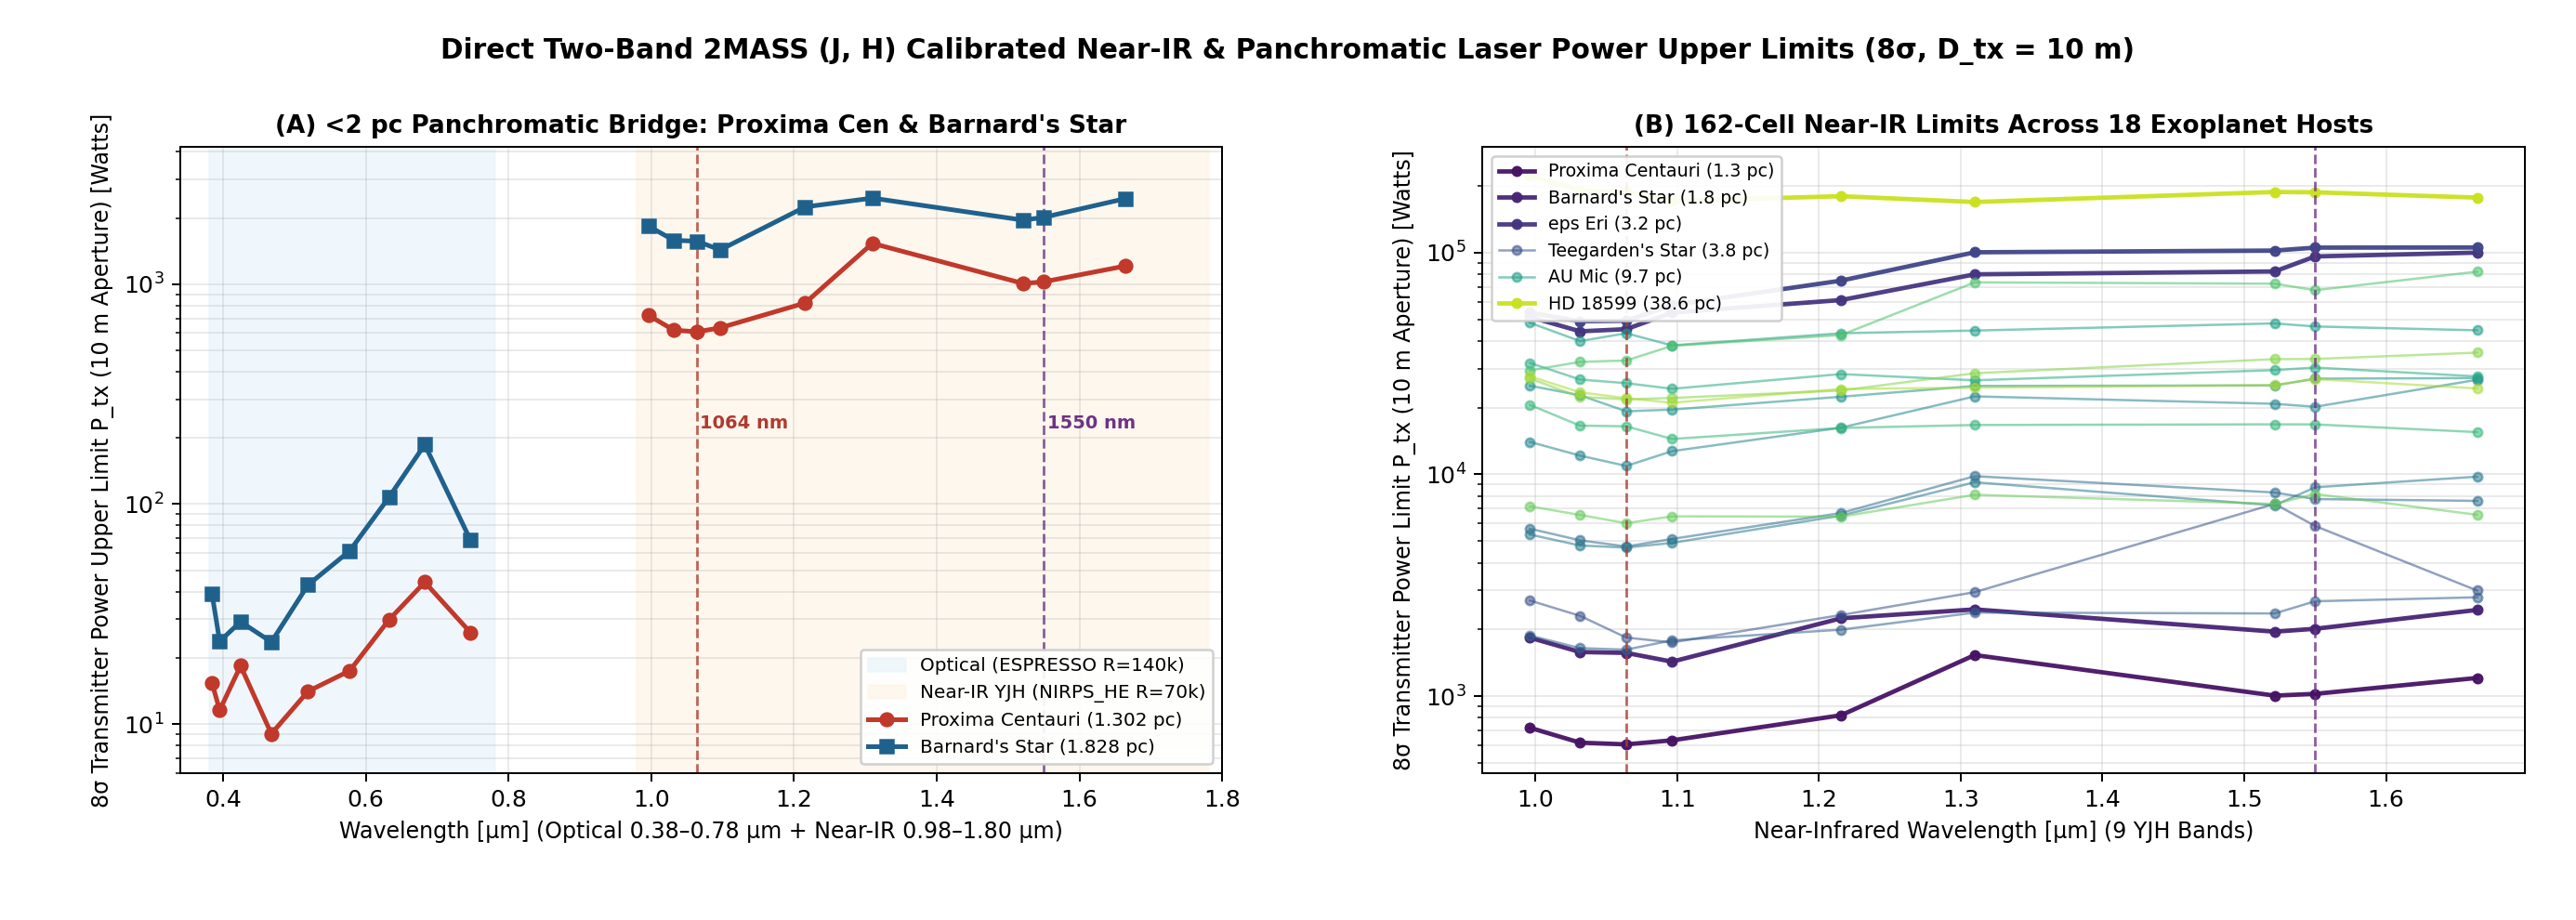
\includegraphics[width=0.80\textwidth]{figures/fig5_panchromatic_2pc_bridge_and_nir_limits.png}
\vspace{0.25em}
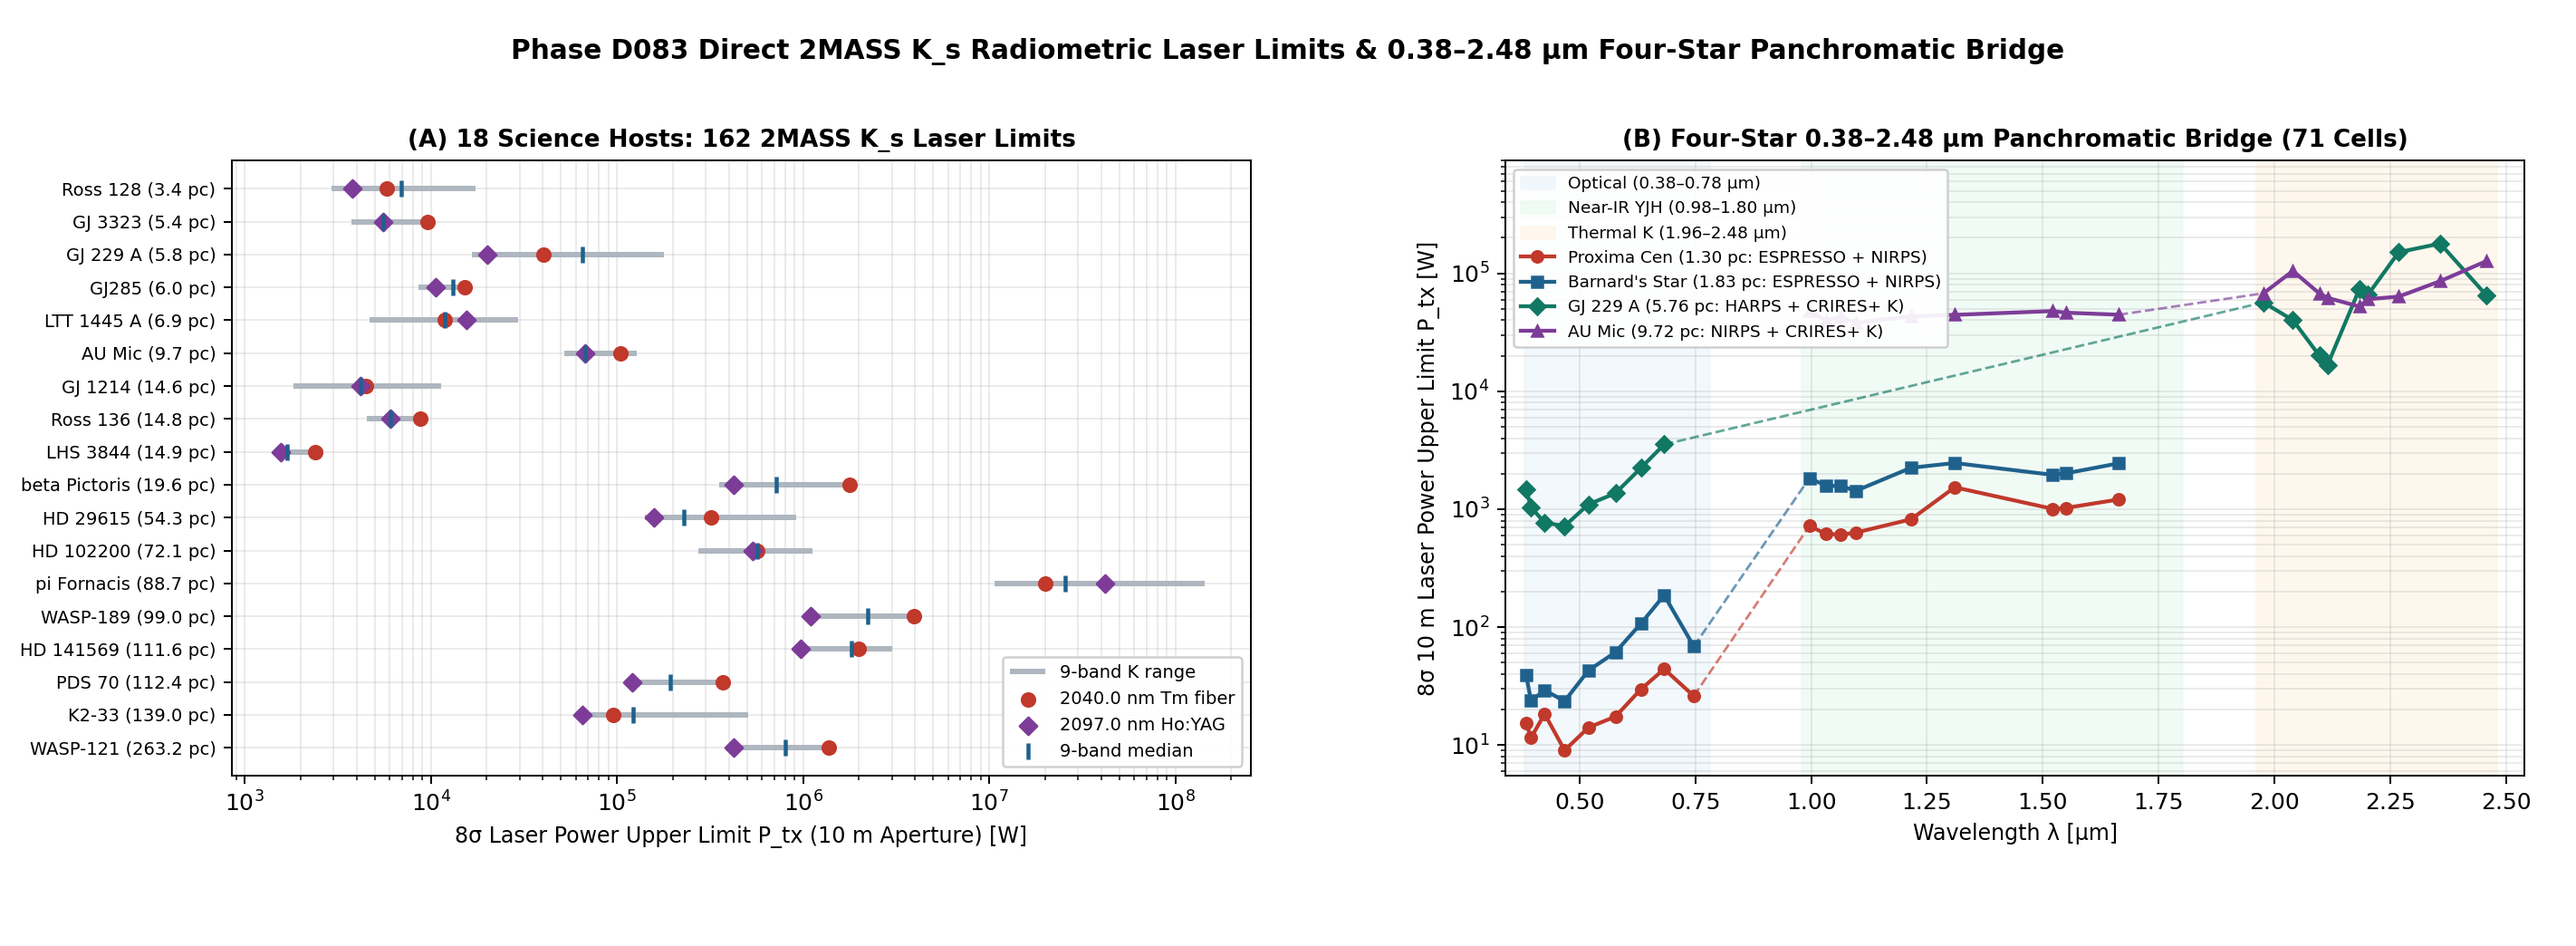
\includegraphics[width=0.84\textwidth]{figures/fig10_kband_laser_limits_and_bridge_spectra.png}
\caption{Spectrophotometrically calibrated CW laser power upper limits ($8\sigma$, $D_{\mathrm{tx}}=10\,\text{m}$): \textbf{Top:} $<2\,\text{pc}$ optical + YJH bridge on Proxima Centauri ($9.03\,\text{W}$ optical; $607.7\,\text{W}$ at $1064.1\,\text{nm}$; $1{,}026.1\,\text{W}$ at $1550.0\,\text{nm}$) and Barnard's Star, alongside 162 YJH limits (\texttt{D082}). \textbf{Bottom:} All 162 2MASS $K_s$-calibrated $K$-band limits across the 18 \texttt{D083} science hosts (down to $1{,}513.2\,\text{W}$ single-epoch and $653.6\,\text{W}$ orbital \texttt{K\_PLANET} on LHS\,3844) and the complete 71-cell four-star $0.38\text{--}2.48\,\mu\text{m}$ panchromatic bridge (Proxima Centauri, Barnard's Star, GJ\,229\,A, AU\,Mic).}
\label{fig:bridge}
\end{figure*}

\begin{figure*}[!t]
\centering
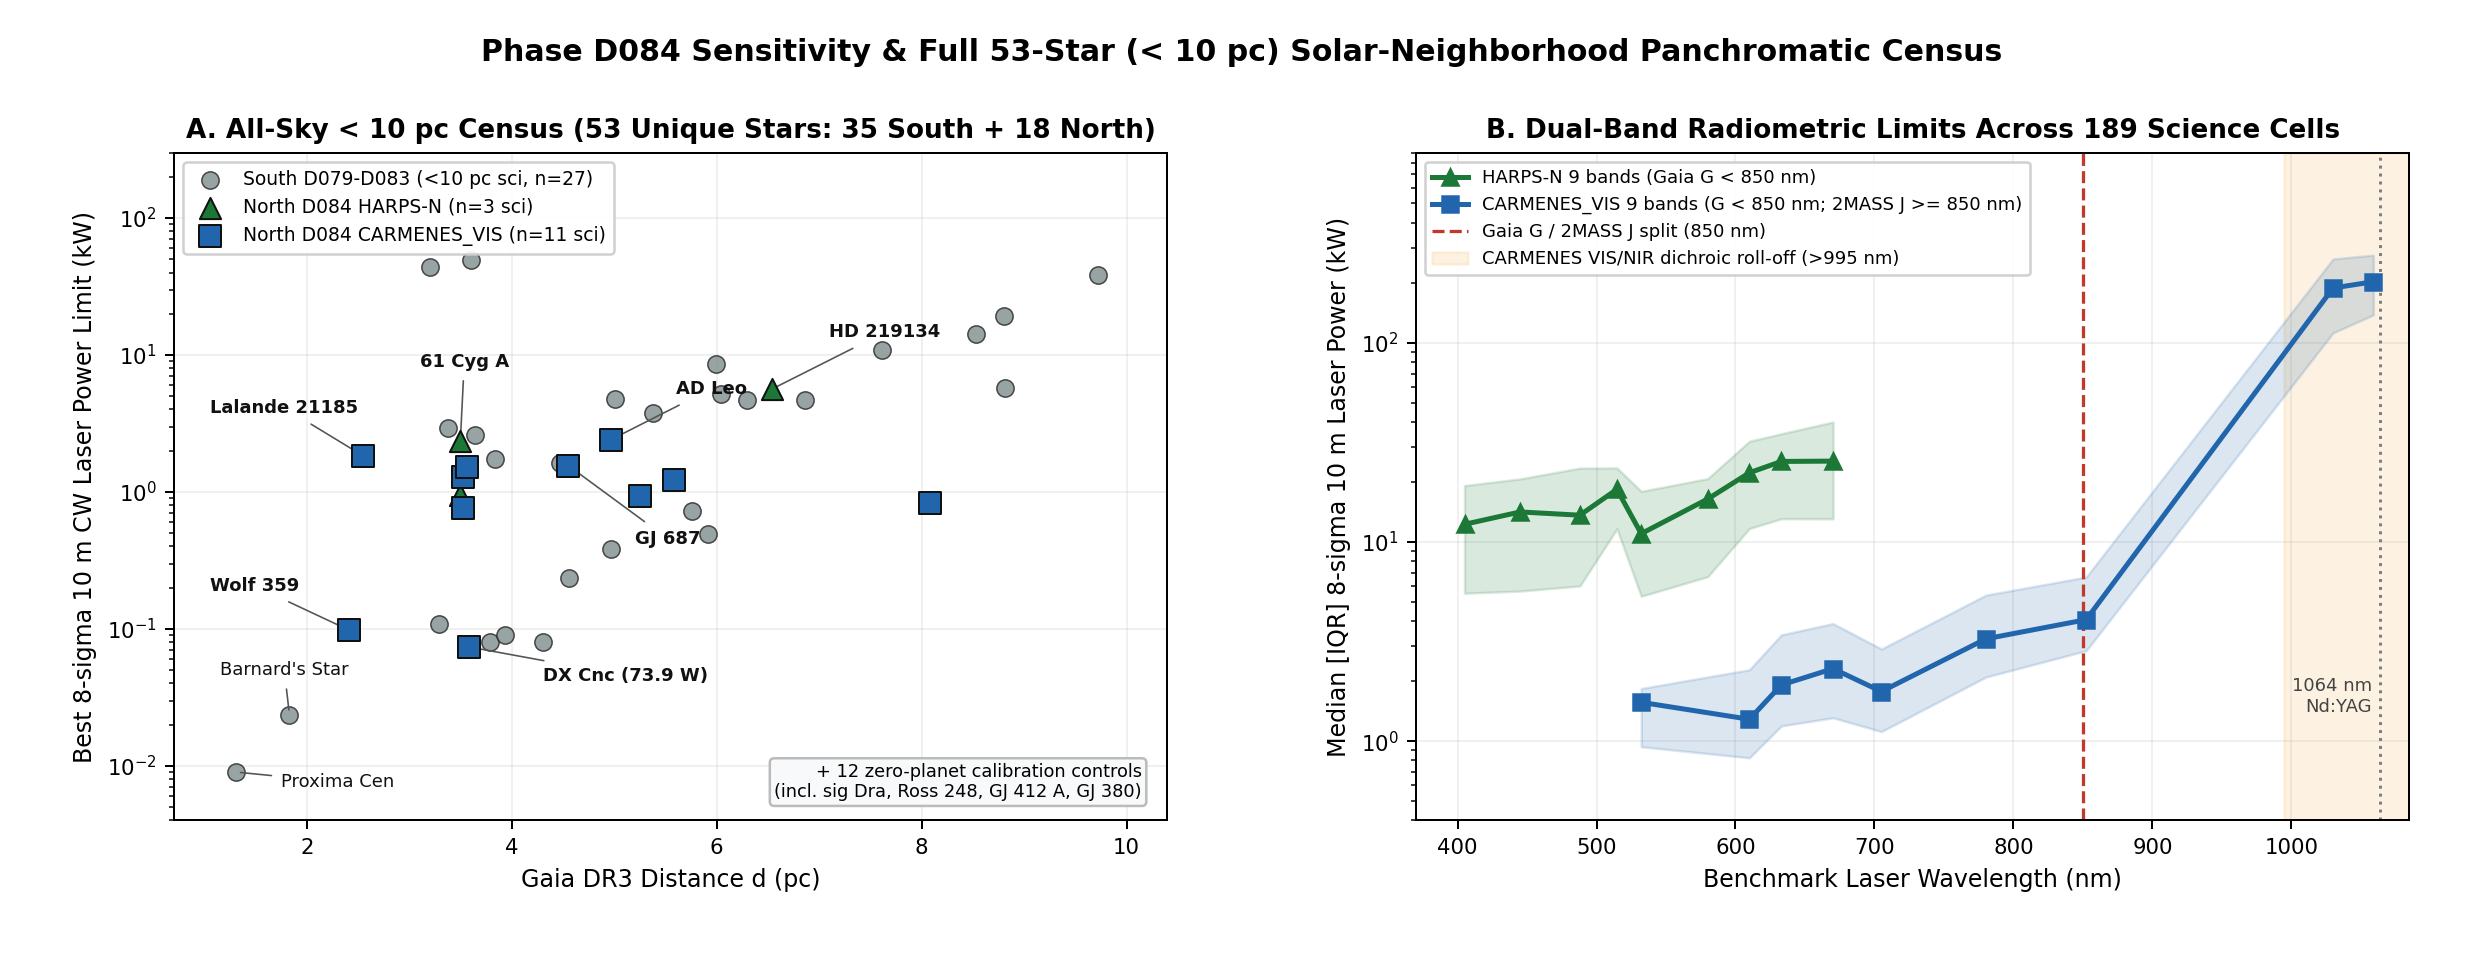
\includegraphics[width=0.90\textwidth]{figures/fig13_allsky_53star_10pc_limits.png}
\vspace{0.25em}
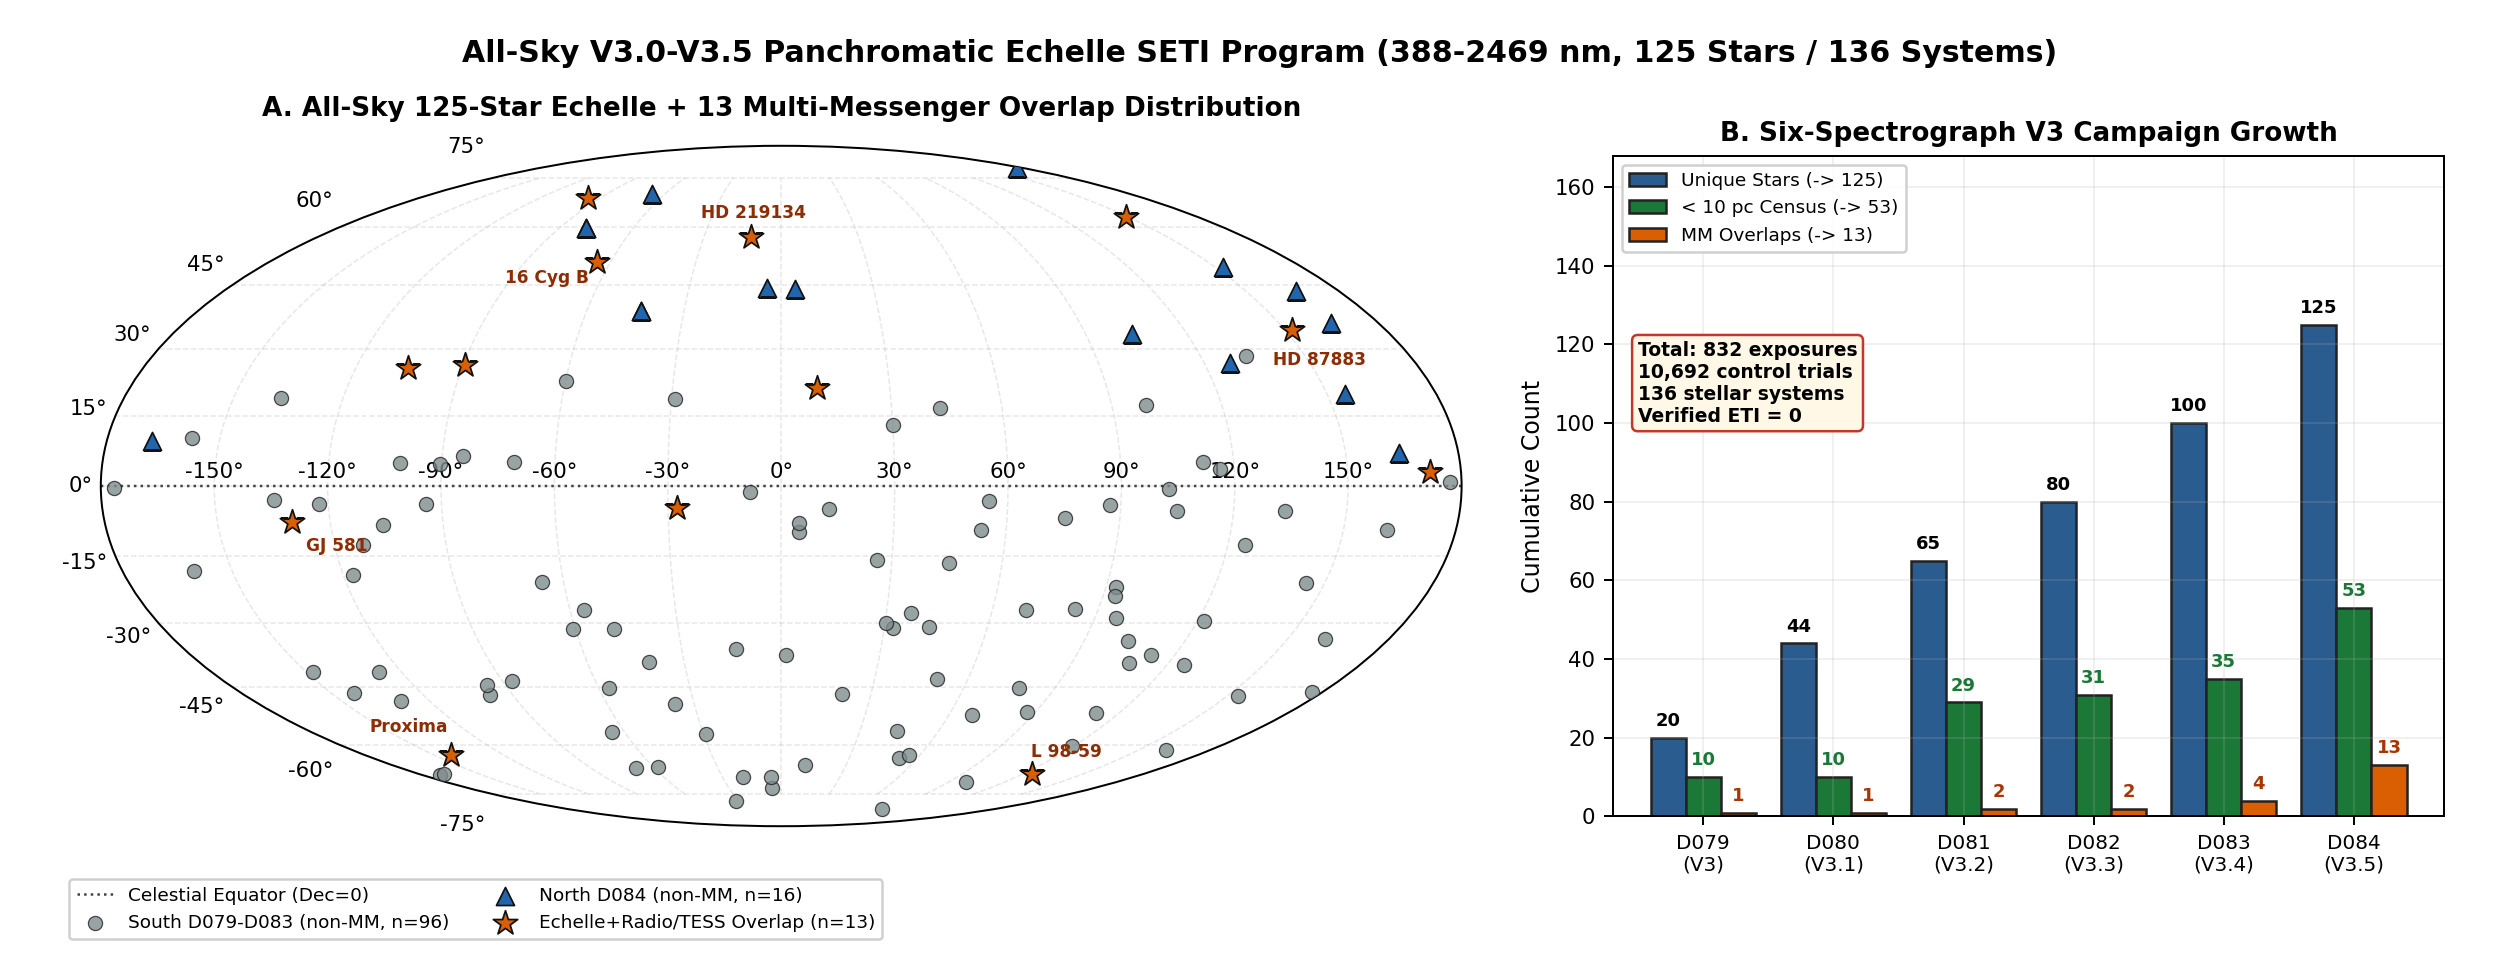
\includegraphics[width=0.92\textwidth]{figures/fig14_allsky_125star_136system_synthesis.png}
\caption{Interim \texttt{D079-D084} 125-star and 189-cell northern optical/dichroic benchmark prior to SPIRou closure: \textbf{Top:} 53-star $<10\,\text{pc}$ subset ($1.62\,\text{kW}$ median) and the 189 CARMENES VIS / HARPS-N upper limits displaying the CARMENES $>995\,\text{nm}$ dichroic throughput roll-off ($188\text{--}202\,\text{kW}$). \textbf{Bottom:} 125-star Mollweide census and 136-system synthesis prior to Phase \texttt{D085}.}
\label{fig:census125}
\end{figure*}

\begin{figure*}[!t]
\centering
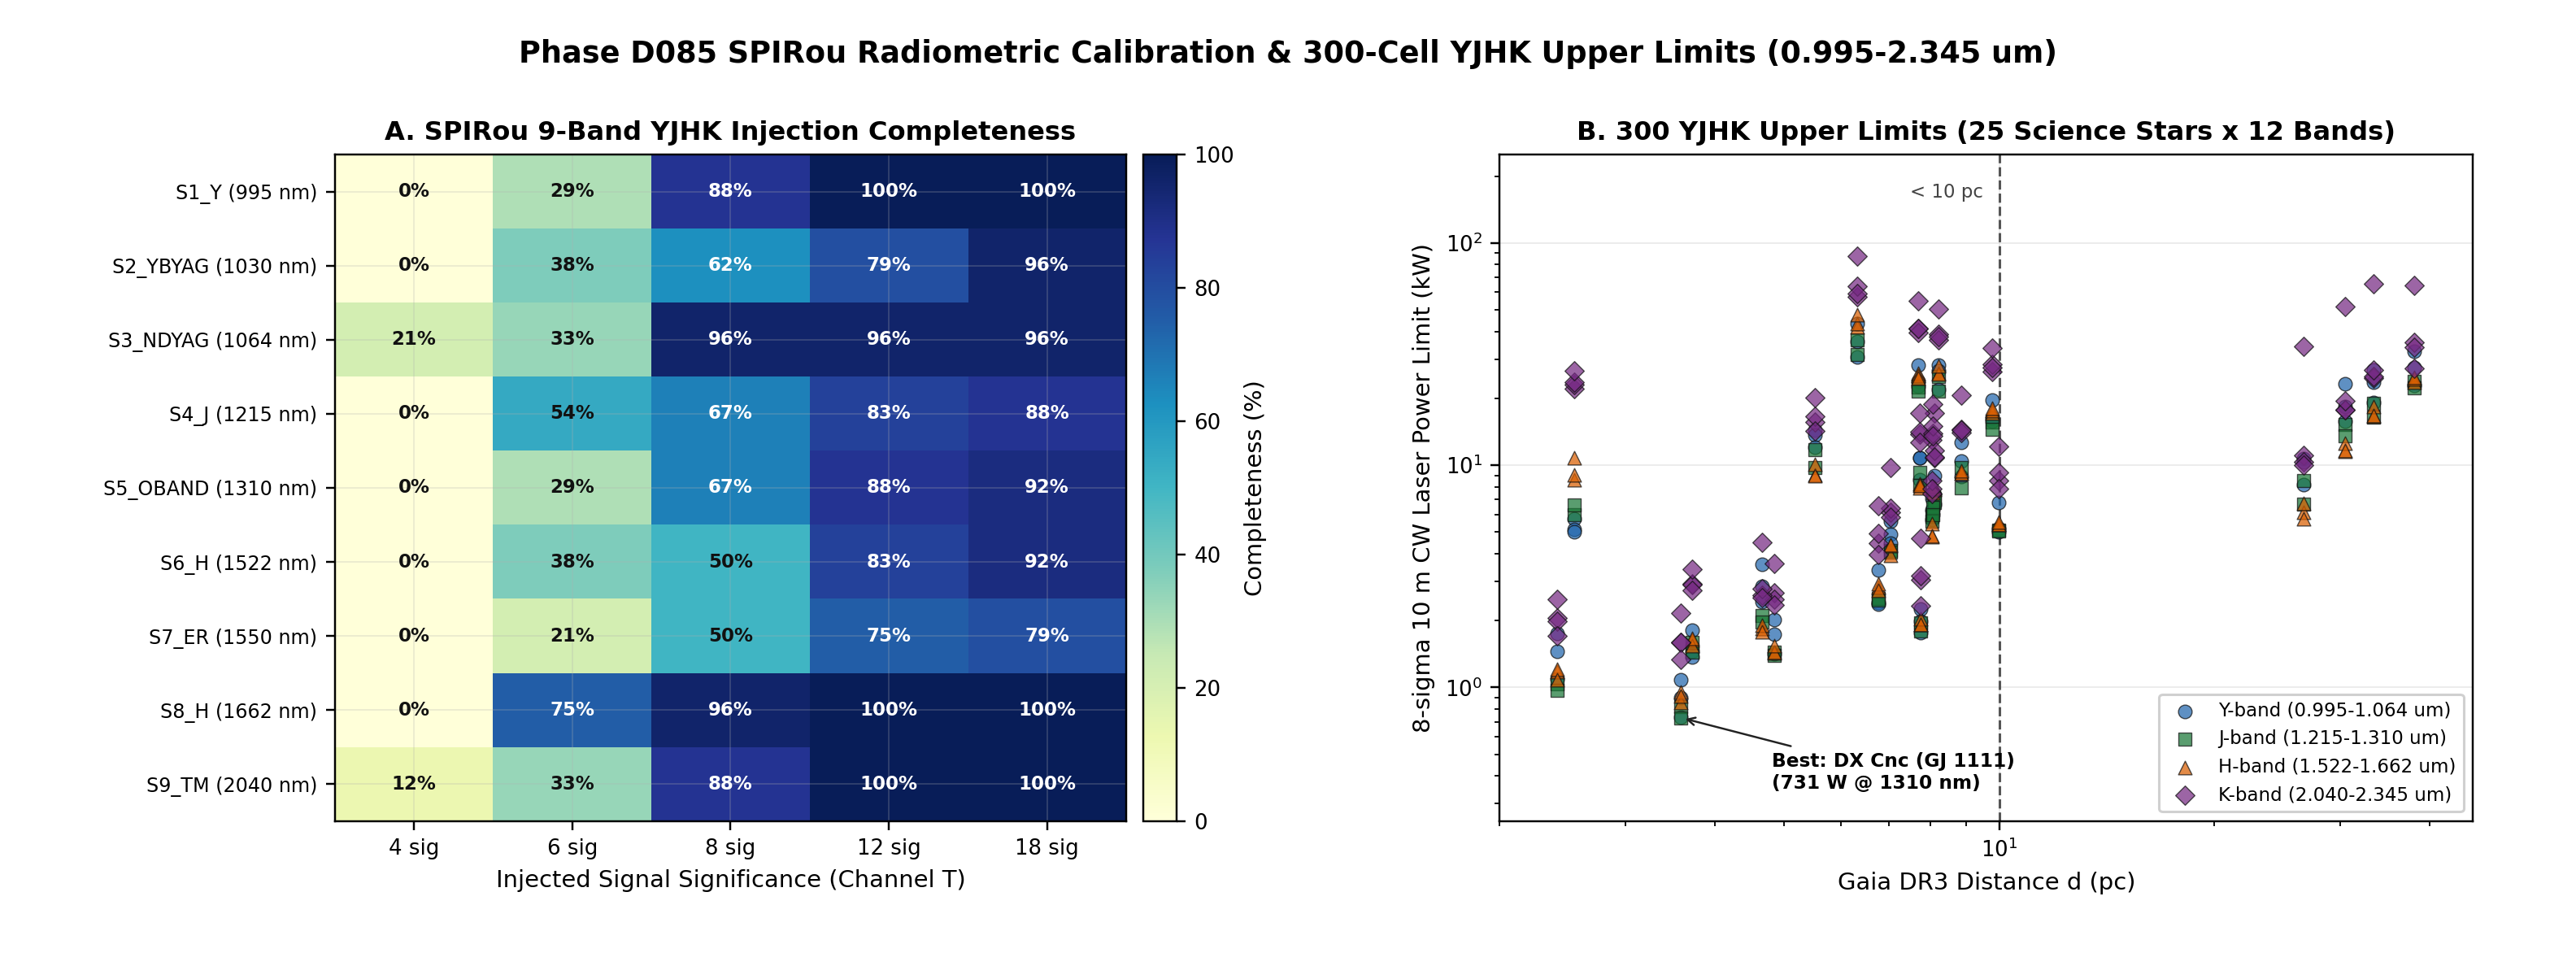
\includegraphics[width=0.88\textwidth]{figures/fig17_d085_yjhk_completeness_and_300_upper_limits.png}
\vspace{0.25em}
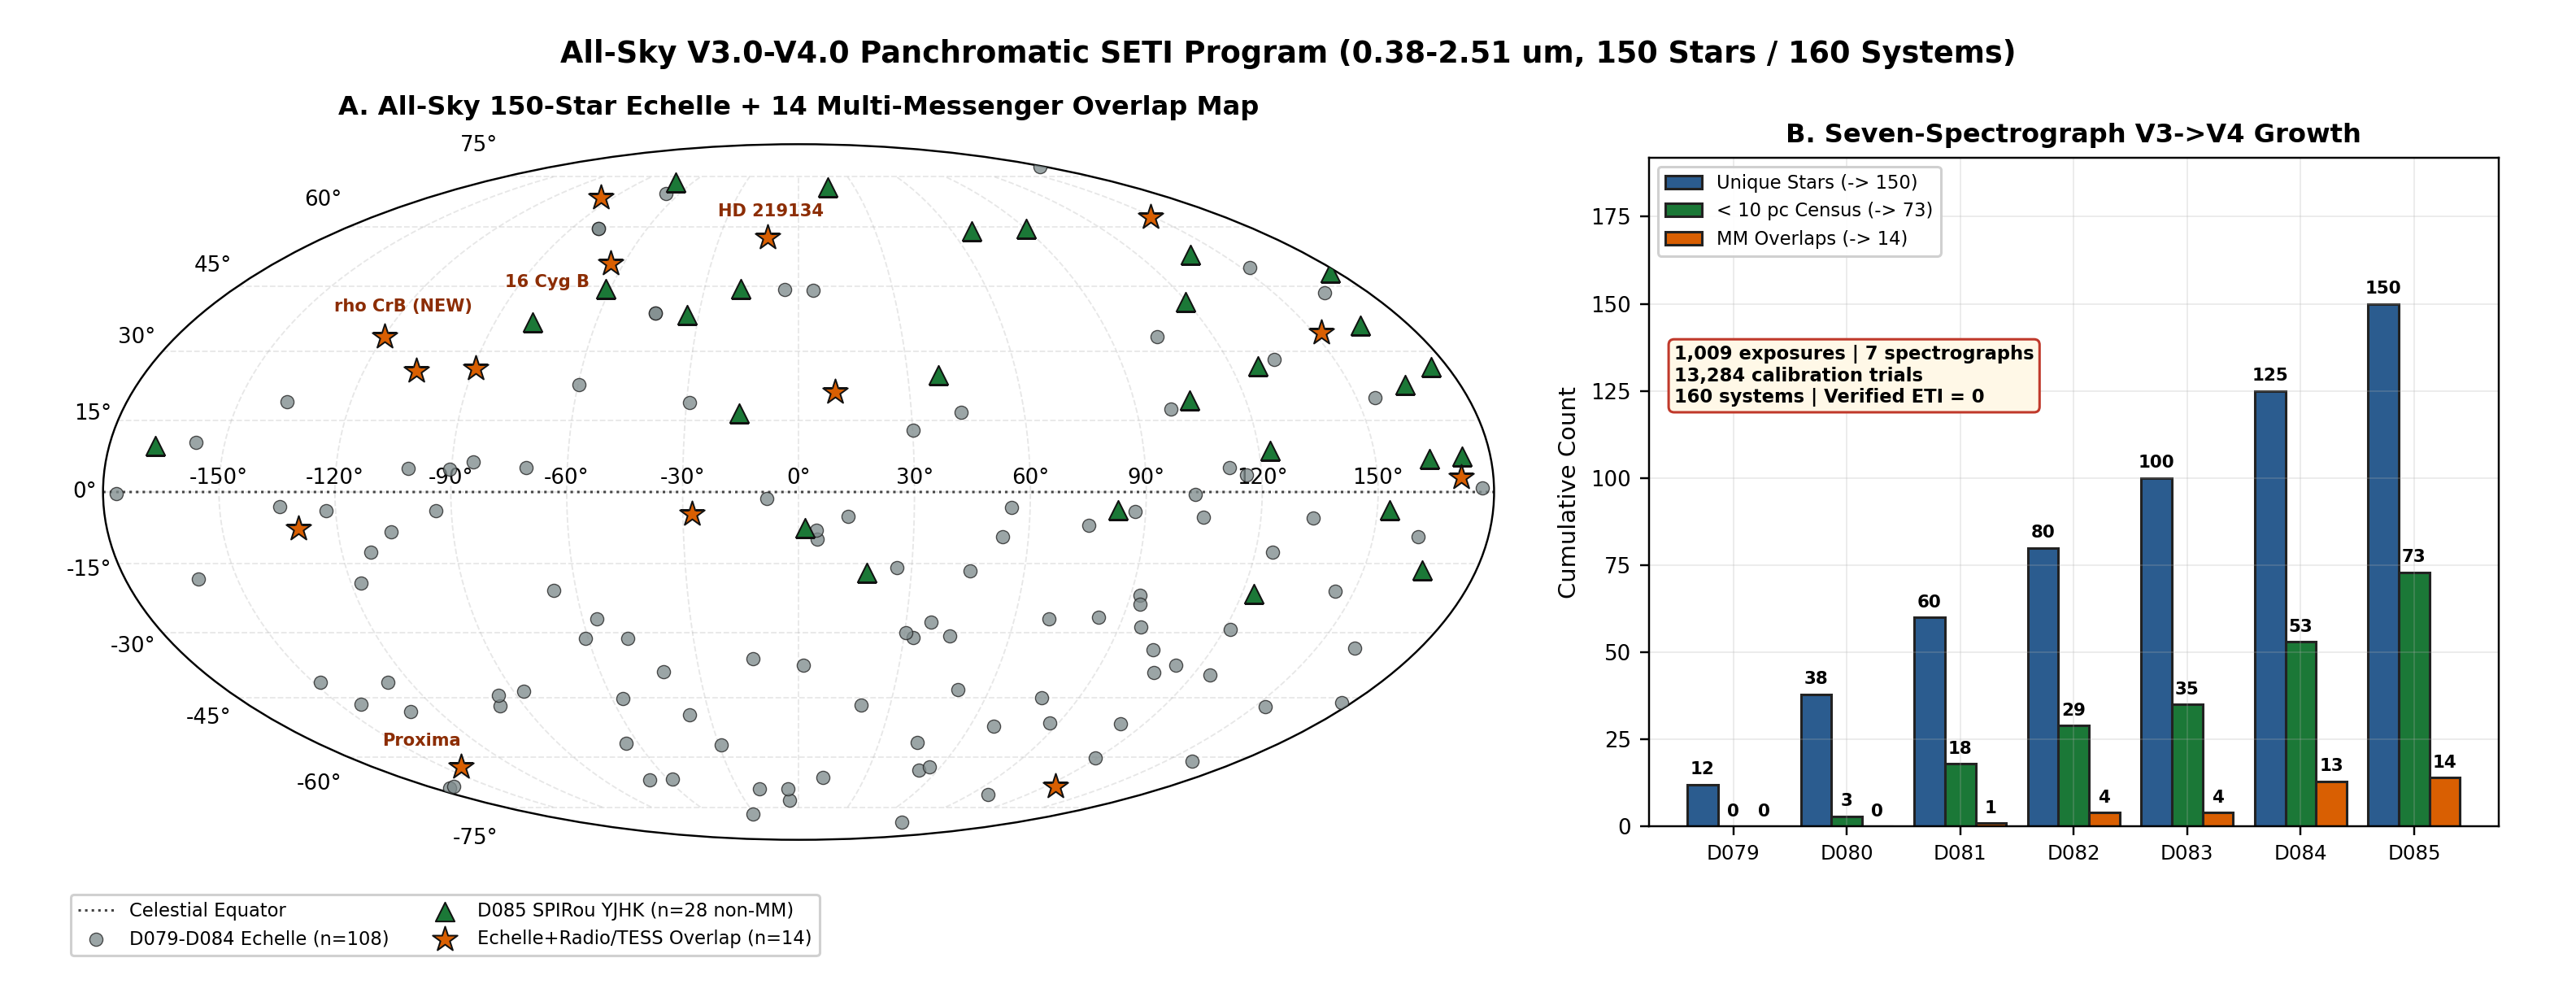
\includegraphics[width=0.90\textwidth]{figures/fig18_d085_allsky_150star_73_10pc_and_160system_synthesis.png}
\caption{Final \texttt{D085} YJHK upper limits and unified 150-star / 160-system all-sky synthesis (\texttt{D079-D085}): \textbf{Top:} Twelve-band $0.995\text{--}2.400\,\mu\text{m}$ SPIRou calibration completeness ($85.5\%$ \texttt{T}, $85.8\%/90.3\%$ \texttt{P}) and all 300 2MASS $(J,H,K_s)$-calibrated $8\sigma$ $10\,\text{m}$ upper limits across the 25 SPIRou science hosts (down to $730.5\,\text{W}$ on DX\,Cnc at $1310\,\text{nm}$ and $972.7\,\text{W}$ on Wolf\,359). \textbf{Bottom:} Complete all-sky Mollweide census of all \textbf{150 unique echelle stars} ($106$ South + $44$ North), \textbf{73} $<10\,\text{pc}$ \textbf{stars} ($2.37\,\text{kW}$ median), \textbf{8 panchromatic bridges} ($155$ cells), \textbf{14 direct overlap hosts} across \textbf{160 distinct multi-messenger systems} (adding $\rho$\,CrB / \texttt{M20}), and seven-phase cumulative growth (1,009 exposures, 13,284 trials, 0 verified ETI).}
\label{fig:census150}
\end{figure*}

\begin{table*}[t]
\centering
\caption{The 18 Northern $<10\,\text{pc}$ Targets Added in \texttt{D084} Together With the Four Northern CARMENES--SPIRou Dichroic Bridge Closures and Expanded 73-Star $<10\,\text{pc}$ Summary Through \texttt{D085}.}
\label{tab:10pc}
\resizebox{\textwidth}{!}{%
\begin{tabular}{llccccccc}
\toprule
Star & Common Name & Instrument & Role & $d$ (pc) & $T_{\mathrm{eff}}$ (K) & $N_{\mathrm{pl}}$ / $N_{\mathrm{exp}}$ & Best $<850\,\text{nm}$ / $\ge 850\,\text{nm}$ $8\sigma$ $10\,\text{m}$ Limit & Verified ETI \\
\midrule
\textbf{WOLF359}      & Wolf\,359 (CN Leo)         & CARMENES\_VIS+SPIRou & Science & 2.409 & 3071 & 0 / 10 & \textbf{98.15\,W} / \textbf{487.8\,W} (\textbf{972.7\,W} $1310\,\text{nm}$) & \textbf{0} \\
\textbf{LALANDE21185} & Lalande\,21185 (GJ\,411)   & CARMENES\_VIS+SPIRou & Science & 2.546 & 3557 & 2 / 20 & 1.84\,kW / \textbf{5.00\,kW} ($1064\,\text{nm}$; \textbf{2.82\,kW} \texttt{K\_PL}) & \textbf{0} \\
\textbf{ROSS248}      & Ross\,248 (HH And)         & CARMENES\_VIS & Control & 3.160 & 3190 & 0 / 12 & Calibration Control (0 FA)                   & \textbf{0} \\
\textbf{61CYGB}       & 61\,Cygni\,B               & HARPS-N       & Science & 3.496 & 4044 & 0 / 5  & \textbf{946.0\,W} / ---                      & \textbf{0}$^{\ast}$ \\
\textbf{61CYGA}       & 61\,Cygni\,A               & HARPS-N       & Science & 3.497 & 4374 & 0 / 5  & 2.36\,kW / ---                               & \textbf{0} \\
\textbf{STRUVE2398A}  & Struve\,2398\,A (Gl\,725\,A) & CARMENES\_VIS & Science & 3.523 & 3470 & 1 / 10 & 1.29\,kW / 4.46\,kW                          & \textbf{0} \\
\textbf{STRUVE2398B}  & Struve\,2398\,B (Gl\,725\,B) & CARMENES\_VIS & Science & 3.523 & 3390 & 1 / 5  & \textbf{759.8\,W} / 2.85\,kW                 & \textbf{0} \\
\textbf{GXAND}        & GX\,And (GJ\,15\,A)        & CARMENES\_VIS & Science & 3.562 & 3603 & 2 / 10 & 1.52\,kW / 3.95\,kW                          & \textbf{0} \\
\textbf{DXCNC}        & DX\,Cnc (GJ\,1111)         & CARMENES\_VIS+SPIRou & Science & 3.581 & 3000 & 0 / 10 & \textbf{73.90\,W} / \textbf{342.2\,W} (\textbf{730.5\,W} $1310\,\text{nm}$) & \textbf{0} \\
\textbf{GJ687}        & GJ\,687 (GBT+Echelle)      & CARMENES\_VIS & Science & 4.550 & 3390 & 2 / 10 & 1.56\,kW / 4.64\,kW                          & \textbf{0} \\
\textbf{HD88230}      & GJ\,380                    & HARPS-N       & Control & 4.871 & 4131 & 0 / 5  & Calibration Control (0 FA)                   & \textbf{0} \\
\textbf{GJ412A}       & GJ\,412\,A                 & CARMENES\_VIS & Control & 4.905 & 3628 & 0 / 5  & Calibration Control (0 FA)                   & \textbf{0} \\
\textbf{ADLEO}        & AD\,Leo (GJ\,388)          & CARMENES\_VIS & Science & 4.965 & 3455 & 0 / 5  & 2.41\,kW / 9.32\,kW                          & \textbf{0} \\
\textbf{GJ445}        & GJ\,445                    & CARMENES\_VIS & Science & 5.254 & 3360 & 0 / 5  & \textbf{941.2\,W} / 2.92\,kW                 & \textbf{0} \\
\textbf{GJ251}        & GJ\,251 (Wolf\,294)        & CARMENES\_VIS & Science & 5.585 & 3500 & 2 / 10 & 1.21\,kW / 4.07\,kW                          & \textbf{0} \\
\textbf{HD185144}     & $\sigma$\,Draconis         & HARPS-N       & Control & 5.764 & 5246 & 0 / 12 & Calibration Control (0 FA)                   & \textbf{0} \\
\textbf{HD219134}     & HD\,219134 (GBT+Echelle)   & HARPS-N       & Science & 6.542 & 4798 & 6 / 12 & 5.65\,kW / ---                               & \textbf{0}$^{\ast}$ \\
\textbf{GJ486}        & GJ\,486 (Wolf\,437)        & CARMENES\_VIS+SPIRou & Science & 8.079 & 3410 & 1 / 17 & \textbf{824.8\,W} (\textbf{357\,W} \texttt{K\_PL}) / 2.84\,kW (\textbf{5.96\,kW} $1064\,\text{nm}$) & \textbf{0}$^{\ast}$ \\
\midrule
\textbf{D085 New $<10\,\text{pc}$ (20)} & 15 North + 5 South & CFHT SPIRou & 16 Sci / 4 Ctrl & 3.72--9.99 & 2865--4014 & 10 pl. & \textbf{1.37\,kW} (YZ\,Cet), \textbf{1.39\,kW} (GJ\,1002), \textbf{718\,W} (\texttt{K\_PL}) & \textbf{0} \\
\textbf{73-Star $<10\,\text{pc}$ Census} & \textbf{40 South + 33 North} & \textbf{All 7 V3--V4 Instr.} & \textbf{57 Sci / 16 Ctrl} & $\mathbf{1.30\text{--}9.99}$ & \textbf{2865--5604} & \textbf{83 pl.} & \textbf{2.37\,kW median (min 9.03\,W Proxima Cen)} & \textbf{0} \\
\bottomrule
\end{tabular}%
}
\par\smallskip\scriptsize{$^{\ast}$Automated post-\texttt{G6} single-epoch \texttt{Channel T} transients in \texttt{D084} ($1$ on 61\,Cyg\,B, $4$ on HD\,219134, $1$ on GJ\,486) forensically confirmed atmospheric/instrumental (\texttt{FORENSIC\_CANDIDATE\_AUDIT\_D084.json}); all $19$ \texttt{COMB\_V4} hits (17 M2V FeH/TiO on Lalande\,21185 + 2 telluric/Al\,I on $\rho$\,CrB) and $113$ single-line hits in \texttt{D085} are 100\% forensically natural (\texttt{FORENSIC\_CANDIDATE\_AUDIT\_D085.json}); $0$ orbital hits.}
\end{table*}

\section{Panchromatic Laser Limits ($0.38\text{--}2.515\,\mu\text{m}$) \& 160-System Synthesis}
For an unresolved Gaussian LSF ($\mathrm{FWHM}_{\mathrm{LSF}} = \lambda/R$) above empirical residual noise $\sigma_{\mathrm{MAD}}$, $\mathrm{EW}_{8\sigma}(\lambda) = \sqrt{\pi/(4\ln 2)}\,(8\sigma_{\mathrm{MAD}})\,\lambda/R$. Anchoring continuum flux $F_{\lambda,\star}(\lambda)$ at Earth to Gaia DR3 ($G_{\mathrm{BP}}, G, G_{\mathrm{RP}}$; \cite{GaiaDR3}) below $850\,\text{nm}$, 2MASS $J$ ($\ge 850\,\text{nm}$ in \texttt{D082/D084/D085}), $H$ (\texttt{D082/D085}), and 2MASS $K_s$ ($2.159\,\mu\text{m}$, $F_{\lambda,0} = 4.283\times 10^{-11}\,\text{erg\,cm}^{-2}\,\text{s}^{-1}\,\text{\AA}^{-1}$; \cite{Cohen2003}) in \texttt{D083/D085} with Planck $B_{\lambda}(T_{\mathrm{eff}})$ intra-band scaling, the $8\sigma$ beamed CW power limit for a $D_{\mathrm{tx}} = 10\,\text{m}$ transmitter is
\begin{equation}
  P_{\mathrm{tx},8\sigma}(D_{\mathrm{tx}}=10\,\text{m}) = 4 d^2 F_{\lambda,\star}(\lambda)\,\mathrm{EW}_{8\sigma}(\lambda)\!\left(\frac{\lambda}{D_{\mathrm{tx}}}\right)^{2},
\end{equation}
scaling as $(10\,\text{m}/D_{\mathrm{tx}})^2$ for any transmitter aperture. Figures~\ref{fig:bridge}--\ref{fig:census150} and Table~\ref{tab:10pc} synthesize our panchromatic and multi-messenger constraints:
\begin{itemize}
  \item \textbf{Eight-Star $0.38\text{--}2.515\,\mu\text{m}$ Panchromatic Bridge (155 Cells) \& Northern Dichroic Closure:} In the south, \textbf{Proxima Centauri} ($1.302\,\text{pc}$) reaches \textbf{9.03\,W} ($467.6\,\text{nm}$), \textbf{607.7\,W} ($1064.1\,\text{nm}$), and \textbf{1,026.1\,W} ($1550.0\,\text{nm}$); \textbf{Barnard's Star} ($1.828\,\text{pc}$) reaches \textbf{23.61\,W} (optical) and \textbf{1,433.0\,W} ($1096.5\,\text{nm}$); \textbf{GJ\,229\,A} links \textbf{720.4\,W} (HARPS) with \textbf{16.64\,kW} $K$-band; and \textbf{AU\,Mic} links \textbf{38.13\,kW} YJH with \textbf{52.30\,kW} $K$-band. In the north, \textbf{D085} SPIRou closes the CARMENES VIS $>995\,\text{nm}$ dichroic roll-off by \textbf{12--51$\times$} across four $<10\,\text{pc}$ bridges: \textbf{DX\,Cnc} drops from $11.12/11.74\,\text{kW}$ ($1030/1059\,\text{nm}$) to \textbf{895\,W} / \textbf{736\,W} ($1064.1\,\text{nm}$) and \textbf{730.5\,W} ($1310\,\text{nm}$); \textbf{Wolf\,359} drops from $14.06/15.85\,\text{kW}$ to \textbf{1.45/1.09\,kW} (\textbf{972.7\,W} at $1310\,\text{nm}$); \textbf{Lalande\,21185} drops $51.3\times$ ($256.8 \rightarrow 5.00\,\text{kW}$; \textbf{2.82\,kW} on GJ\,411\,b); and \textbf{GJ\,486} drops $26.6\times$ ($158.9 \rightarrow 5.96\,\text{kW}$).
  \item \textbf{Expanded 73-Star $<10\,\text{pc}$ Census \& 300 SPIRou Limits:} Adding 20 new $<10\,\text{pc}$ targets in \texttt{D085} (16 science + 4 controls) brings the $<10\,\text{pc}$ census to \textbf{73 stars} (57 science hosts including 41 planet hosts with 83 planets + 16 controls), with a median best $8\sigma$ $10\,\text{m}$ limit of \textbf{2.3716\,kW} (\textbf{7.8493\,kW} median across all 124 science stars). Top new YJHK single-epoch limits include \textbf{DX\,Cnc} (\textbf{730.5\,W}), \textbf{Wolf\,359} (\textbf{972.7\,W}), \textbf{YZ\,Cet} (\textbf{1,369.4\,W} at $1064.1\,\text{nm}$), and \textbf{GJ\,1002} (\textbf{1,393.4\,W} at $1310\,\text{nm}$), alongside orbital \texttt{K\_PLANET} bounds of \textbf{718\,W} (\textbf{GJ\,1002\,b}) and \textbf{736\,W} (\textbf{YZ\,Cet\,b}).
  \item \textbf{160-System Multi-Messenger Synthesis:} Uniting the 150-star all-sky echelle atlas with 23 exoplanet systems searched at $1.4\,\text{GHz}$ on Parkes 64\,m and GBT 100\,m (\texttt{M5-M36}; \texttt{M35} $95\%$ bound \textbf{33.16\%} at $\mathrm{SNR}=40$) and TESS light-sail vetting on L\,98-59 (\texttt{LS7}) yields \textbf{160 distinct stellar systems} (136 echelle-only + 10 radio-only + \textbf{14 direct multi-messenger overlap hosts}: Proxima Cen, GJ\,581, GJ\,849, L\,98-59, 9 northern \texttt{D084} GBT hosts, and $\rho$\,CrB [\texttt{M20}]; Fig.~\ref{fig:census150}) with \textbf{0 verified ETI detections}.
\end{itemize}

\section{Conclusions}
Across seven prospectively locked echelle phases spanning $0.38\text{--}2.515\,\mu\text{m}$ on seven spectrographs across both hemispheres (HARPS, ESPRESSO, NIRPS\_HE, CRIRES+, HARPS-N, CARMENES\_VIS, CFHT SPIRou; 150 unique stars, 1,009 exposures, $195.23\,\text{h}$, 13,284 calibration trials, $221.66\times 10^{6}$ 1D bins + $20.92\times 10^{6}$ \texttt{COMB\_V4} configurations) unified with 23 planet-frame $1.4\,\text{GHz}$ radio hosts and TESS photometry (160 distinct systems total, 14 direct overlap hosts), physics-based five-channel vetting and sparse cross-star coincidence gating (\texttt{G6\_V36}; $95.0\%$ true-laser pass at $100\%$ OH/warm-pixel/BERV-stationary rejection) eliminate 12,107 Legacy \texttt{V2} false alarms to \textbf{0 orbital hits} across 40 campaigns and \textbf{0 verified ETI detections}, achieving Watt-to-kilowatt CW and frequency-comb sensitivity across the 73-star $<10\,\text{pc}$ census ($2.37\,\text{kW}$ median; $9.03\,\text{W}$ optical; $730.5\,\text{W}$ northern YJHK). Extending \texttt{COMB\_V4} across all 150 archival optical--$K$ spectra and deep optical coverage ($<10\,\text{W}$) of YJHK-only northern M dwarfs remain natural next steps.

\clearpage
\section*{Data and Code Availability}
All observational data are publicly available via the ESO Science Archive (\texttt{HARPS, ESPRESSO, NIRPS, CRIRES+}), INAF IA2 TNG Archive (\texttt{HARPS-N}), GAVO CARMENES DR1 (\texttt{CARMENES\_VIS}), CADC CFHT Science Archive (\texttt{SPIRou} APERO \texttt{0.7.295}), Breakthrough Listen (Parkes/GBT), MAST (TESS), ESA Gaia DR3, 2MASS, and the NASA Exoplanet Archive (\texttt{obs\_release\_date <= '2026-11-16T00:00:00Z'}). All locked source codes, cryptographic lock receipts, provenance manifests (\texttt{SOURCES.json}), forensic audits (\texttt{FORENSIC\_CANDIDATE\_AUDIT\_D085.json}), synthesis CSVs (\texttt{150STARS}, \texttt{73STARS}, \texttt{160SYSTEMS}, \texttt{BRIDGE\_8STARS}), and pure-stdlib \texttt{python3 -S} audit suites are archived at \url{https://github.com/andersenmartin-blip/setisearch}.

\begin{thebibliography}{99}
\footnotesize
\setlength{\itemsep}{1.2pt}
\bibitem{SchwartzTownes1961} Schwartz, R.~N., \& Townes, C.~H.\ 1961, \textit{Nature}, 190, 205
\bibitem{Townes1983} Townes, C.~H.\ 1983, \textit{PNAS}, 80, 1147
\bibitem{Rousselot2000} Rousselot, P., Lidman, C., Cuby, J.-G., et al.\ 2000, \textit{A\&A}, 354, 1134
\bibitem{Kingsley2001} Kingsley, S.~A.\ 2001, \textit{SPIE Proc.}, 4273, 72
\bibitem{ReinesMarcy2002} Reines, A.~E., \& Marcy, G.~W.\ 2002, \textit{PASP}, 114, 416
\bibitem{Mayor2003} Mayor, M., Pepe, F., Queloz, D., et al.\ 2003, \textit{The Messenger}, 114, 20
\bibitem{Cohen2003} Cohen, M., Wheaton, W.~A., \& Megeath, S.~T.\ 2003, \textit{AJ}, 126, 1090
\bibitem{Howard2004} Howard, A.~W., Horowitz, P., Wilkinson, D.~T., et al.\ 2004, \textit{ApJ}, 613, 1270
\bibitem{Fuhrmeister2011} Fuhrmeister, B., Lalitha, S., Poppenhaeger, K., et al.\ 2011, \textit{A\&A}, 534, A133
\bibitem{TellisMarcy2015} Tellis, N.~K., \& Marcy, G.~W.\ 2015, \textit{PASP}, 127, 540
\bibitem{Oliva2015} Oliva, E., Origlia, L., Scuderi, S., et al.\ 2015, \textit{A\&A}, 581, A47
\bibitem{KippingTeachey2016} Kipping, D.~M., \& Teachey, A.\ 2016, \textit{MNRAS}, 459, 1233
\bibitem{Bouchy2017} Bouchy, F., Doyon, R., Artigau, \'{E}., et al.\ 2017, \textit{The Messenger}, 169, 21
\bibitem{TellisMarcy2017} Tellis, N.~K., \& Marcy, G.~W.\ 2017, \textit{AJ}, 153, 251
\bibitem{Lipman2019} Lipman, E.~A., Isaacson, H., Siemion, A.~P.~V., et al.\ 2019, \textit{PASP}, 131, 034202
\bibitem{Maire2019} Maire, J., Wright, S.~A., Dorval, P., et al.\ 2019, \textit{AJ}, 158, 203
\bibitem{Donati2020} Donati, J.-F., Kouach, D., Moutou, C., et al.\ 2020, \textit{MNRAS}, 498, 5684
\bibitem{Sheikh2020} Sheikh, S.~Z., Wright, J.~T., Siemion, A., \& Enriquez, J.~E.\ 2020, \textit{ApJ}, 888, 78
\bibitem{Pepe2021} Pepe, F., Cristiani, S., Rebolo, R., et al.\ 2021, \textit{A\&A}, 645, A96
\bibitem{Cook2022} Cook, N.~J., Artigau, \'{E}., Doyon, R., et al.\ 2022, \textit{PASP}, 134, 114509
\bibitem{Marcy2022} Marcy, G.~W., Tellis, N.~K., \& Wishnow, E.~H.\ 2022, \textit{MNRAS}, 509, 3798
\bibitem{Dorn2023} Dorn, R.~J., Bristow, P., Smoker, J.~V., et al.\ 2023, \textit{A\&A}, 671, A24
\bibitem{GaiaDR3} Gaia Collaboration, Vallenari, A., Brown, A.~G.~A., et al.\ 2023, \textit{A\&A}, 674, A1
\bibitem{Zuckerman2023} Zuckerman, A., Isaacson, H., Siemion, A.~P.~V., et al.\ 2023, \textit{AJ}, 165, 114
\bibitem{Bouchy2025} Bouchy, F., Artigau, \'{E}., Wildi, F., et al.\ 2025, \textit{A\&A}, NIRPS commissioning
\end{thebibliography}

\end{document}
